\documentclass{ieeeaccess}

\usepackage{spotcolor}

% Bold font setup for ieeeaccess
\makeatletter
\AtBeginDocument{\DeclareMathVersion{bold}
\SetSymbolFont{operators}{bold}{T1}{times}{b}{n}
\SetSymbolFont{NewLetters}{bold}{T1}{times}{b}{it}
\SetMathAlphabet{\mathrm}{bold}{T1}{times}{b}{n}
\SetMathAlphabet{\mathit}{bold}{T1}{times}{b}{it}
\SetMathAlphabet{\mathbf}{bold}{T1}{times}{b}{n}
\SetMathAlphabet{\mathtt}{bold}{OT1}{pcr}{b}{n}
\SetSymbolFont{symbols}{bold}{OMS}{cmsy}{b}{n}
\renewcommand\boldmath{\@nomath\boldmath\mathversion{bold}}}
\makeatother

\def\BibTeX{{\rm B\kern-.05em{\sc i\kern-.025em b}\kern-.08em
    T\kern-.1667em\lower.7ex\hbox{E}\kern-.125emX}}

\usepackage[utf8]{inputenc}
\usepackage[spanish,es-tabla]{babel}
\usepackage{booktabs}
\usepackage{graphicx}
\usepackage{subcaption}
\usepackage{amsmath}
\usepackage{amssymb}
\usepackage{multirow}
\usepackage{url}
\usepackage{cite}
\usepackage{float}
\usepackage{tabularx}
\usepackage{array}

% Definición de comandos personalizados
\newcommand{\at}[1]{@#1}

\begin{document}
\history{Date of publication August 01, 2026, date of current version August 01, 2026.}
\doi{10.1109/ACCESS.2026.0429000}

% ==============================================================================
% TÍTULO Y AUTORES
% ==============================================================================
\title{Benchmark Multi-Criterio de Paradigmas de Filtrado Colaborativo para Recomendación de Literatura Científica: Un Estudio de Robustez y Generalización}

\author{\uppercase{Xavier Peña}\authorrefmark{1} Y
\uppercase{Diego Rivera}\authorrefmark{2}}
\address[1]{carrera de Computación, Facultad de Ingeniería, Universidad de Cuenca, Cuenca 010150, Ecuador (e-mail: xavier.pena@ucuenca.edu.ec)}
\address[2]{Universidad Politécnica Salesiana, Cuenca 010105, Ecuador (e-mail: driverag2@est.ups.edu.ec)}
\tfootnote{Ambos autores contribuyeron equitativamente a este trabajo. D. Rivera es también Vicepresidente de la Sociedad de Tecnología Vehicular (VTS) de IEEE Sección Ecuador.}
\corresp{Autor de correspondencia: Xavier Peña (e-mail: xavier.pena@ucuenca.edu.ec).}

\markboth
{Peña y Rivera: Benchmark Multi-Criterio de Paradigmas de Filtrado Colaborativo}
{Peña y Rivera: Benchmark Multi-Criterio de Paradigmas de Filtrado Colaborativo}



% ==============================================================================
% RESUMEN (ABSTRACT)
% ==============================================================================
\begin{abstract}
El crecimiento acelerado de la producción de literatura científica dificulta que la comunidad investigadora identifique manuscritos relevantes dentro de su dominio de estudio. Aunque los sistemas de recomendación (SR) basados en filtrado colaborativo implícito constituyen una solución establecida para este problema, la literatura especializada presenta frecuentemente evaluaciones fragmentadas que omiten compensaciones de ingeniería (trade-offs) o que carecen de justificaciones estadísticas sobre la variabilidad de los resultados. Este artículo aborda dicha brecha mediante un estudio comparativo multi-criterio y multidimensional de seis familias algorítmicas representativas (incluyendo métodos basados en memoria, redes neuronales profundas, grafos y Transformers). Los modelos son evaluados bajo un protocolo experimental unificado que combina esquemas de evaluación Leave-One-Out (LOO) con preservación de orden cronológico y Random Split 80/10/10 (RS) sobre tres conjuntos de datos reales e independientes: CiteULike-a, CiteULike-t y BibSonomy (36 condiciones experimentales en total). La comparación trasciende las métricas tradicionales de precisión del ranking (Recall, Ganancia Acumulativa Descontada Normalizada [Normalized Discounted Cumulative Gain, NDCG], Rango Recíproco Medio [Mean Reciprocal Rank, MRR]), analizando la cobertura del catálogo, el índice de Gini, el sesgo de popularidad, los costos computacionales en VRAM y throughput de inferencia (usuarios/s), y la sensibilidad de los modelos ante la reducción de datos de entrenamiento, incluyendo el cold-start parcial inducido (mediante simulaciones de reducción al 50\% y 20\%). Los resultados en precisión de ranking, analizados en NDCG\at{10} mediante la prueba de Friedman ($\chi^2 = 26.00, df = 5, p < 0.001$) sobre $N=6$ condiciones independientes y el test de Nemenyi ($\alpha = 0.05$), sugieren diferencias globales significativas bajo la semilla única evaluada, revelando que ningún paradigma prevalece uniformemente en todas las dimensiones y requiriendo cautela en la generalización por la varianza de inicialización. Si bien MultiVAE y NeuMF obtienen la mayor precisión en colecciones de mayor volumen de interacciones, presentan una elevada concentración en artículos populares y una alta sensibilidad a la reducción de datos de entrenamiento. Por su parte, LightGCN y SASRec presentan una menor sensibilidad combinada a la escasez y al cold-start parcial inducido, mientras que ItemKNN registra el menor costo computacional y la mayor diversidad intra-lista, posicionándose como un baseline de referencia relevante para infraestructuras con recursos restringidos.
\end{abstract}

\begin{keywords}
Sistemas de recomendación, literatura científica, filtrado colaborativo, redes neuronales sobre grafos, Transformers, robustez, análisis estadístico.
\end{keywords}

\titlepgskip=-21pt
\maketitle

% ==============================================================================
% 1. INTRODUCCIÓN
% ==============================================================================
\section{Introducción}
\IEEEPARstart{E}{l} volumen de publicaciones científicas y técnicas se incrementa de forma continua, saturando los canales tradicionales de difusión académica. Esta sobrecarga informativa plantea un desafío operativo para investigadores y estudiantes, quienes deben invertir tiempo considerable en la identificación de trabajos relevantes para sus líneas de investigación. En este contexto, los sistemas de recomendación (SR) de literatura científica ofrecen una solución para personalizar el flujo de descubrimiento de artículos a partir de las interacciones previas de los usuarios.

El escenario predominante en la recomendación de artículos académicos es el \emph{filtrado colaborativo con retroalimentación implícita} (implicit feedback). A diferencia de los entornos comerciales con calificaciones explícitas (por ejemplo, evaluaciones de 1 a 5 estrellas), la señal disponible en gestores de referencias o plataformas de marcadores sociales consiste en eventos binarios (tales como guardar un artículo en una carpeta personal, descargarlo o leerlo). El modelado matemático de esta señal implícita presenta dos retos principales: en primer lugar, se carece de retroalimentación negativa directa, dado que la ausencia de interacción no implica necesariamente desinterés, sino desconocimiento del artículo; en segundo lugar, la matriz de interacciones usuario-ítem exhibe una dispersión extrema (sparsity), con densidades que frecuentemente se ubican por debajo del 0.5\%.

Para hacer frente a estos retos, la comunidad de aprendizaje de máquina ha propuesto diversas familias de modelos:
\begin{itemize}
    \item \textbf{ItemKNN:} Representa el enfoque heurístico basado en memoria~\cite{sarwar2001item}. Calcula similitudes estadísticas de co-ocurrencia sobre las columnas de interacción sin requerir parámetros entrenables, sirviendo como control de eficiencia.
    \item \textbf{NeuMF (Neural Matrix Factorization):} Combina factorización de matrices generalizada con redes densas feed-forward~\cite{he2017neural}, reemplazando el producto interno tradicional por representaciones no lineales aprendidas.
    \item \textbf{MultiVAE:} Modela el historial de interacciones del usuario como una muestra proveniente de una distribución multinomial latente mediante un autoencoder variacional~\cite{liang2018variational}.
    \item \textbf{SASRec y BERT4Rec:} Utilizan mecanismos de autoatención (Transformers) unidireccionales~\cite{kang2018self} y bidireccionales~\cite{sun2019bert4rec} respectivamente, asumiendo una dinámica de lectura secuencial.
    \item \textbf{LightGCN:} Simplifica la propagación en grafos bipartitos al eliminar transformaciones lineales de pesos y activaciones no lineales~\cite{he2020lightgcn}, realizando agregaciones de embeddings entre nodos vecinos.
\end{itemize}

A pesar del acelerado desarrollo de estas arquitecturas, estudios recientes señalan que las evaluaciones experimentales del área tienden a concentrarse únicamente en la precisión del ranking offline (como NDCG\at{10}), omitiendo análisis de reproducibilidad o comparaciones sistemáticas frente a baselines heurísticos bien calibrados, como argumentan Dacrema et al.~\cite{dacrema2019really} y Petrov y Macdonald~\cite{petrov2023effective}. Asimismo, aspectos de ingeniería como el consumo de memoria, el throughput de inferencia o la degradación de rendimiento ante datos escasos no suelen integrarse en un marco de evaluación unificado.

Para abordar estas limitaciones, este estudio presenta un análisis comparativo multidimensional de las seis familias de modelos sobre tres colecciones de datos independientes (CiteULike-a, CiteULike-t y BibSonomy). El trabajo examina cuatro preguntas de investigación principales:

\begin{itemize}
    \item \textbf{RQ1 (Precisión vs. Complejidad):} ¿Muestran los modelos basados en aprendizaje profundo un incremento estadísticamente significativo en la precisión del ranking respecto a baselines heurísticos bien optimizados?
    \item \textbf{RQ2 (Consistencia entre Colecciones):} ¿Se mantienen constantes los ránkings de desempeño de los algoritmos al evaluar sobre colecciones con diferentes niveles de densidad y volumen de interacciones?
    \item \textbf{RQ3 (Sensibilidad a la Reducción de Datos de Entrenamiento):} ¿En qué medida se degrada la precisión de cada modelo al reducir la información de entrenamiento al 50\% y 20\% manteniendo constante el conjunto de evaluación?
    \item \textbf{RQ4 (Compensaciones Multi-Criterio):} ¿Existe un algoritmo dominante en todas las dimensiones evaluadas, o se observan compensaciones (trade-offs) entre precisión, diversidad, resiliencia y costo computacional?
\end{itemize}

% ==============================================================================
% 2. ESTADO DEL ARTE Y TRABAJO RELACIONADO
% ==============================================================================
\section{Estado del Arte y Trabajo Relacionado}
\label{sec:estado_arte}

La recomendación de literatura científica ha evolucionado desde sistemas basados en procesamiento de lenguaje natural y filtrado por contenido (Content-Based Filtering) hasta enfoques colaborativos profundos basados en representaciones latentes. En esta sección se examinan las tres vertientes fundamentales en las que se enmarca esta investigación.

\subsection{Filtrado Colaborativo Implícito en Literatura Académica}
A diferencia de los dominios de entretenimiento o comercio electrónico (donde plataformas como Netflix o Amazon disponen de calificaciones explícitas o clics frecuentes), el dominio académico se caracteriza por interacciones implícitas de baja frecuencia pero alta especificidad temática. Hu et al.~\cite{hu2008collaborative} y Koren et al.~\cite{koren2009matrix} formalizaron los modelos de factorización de matrices implícita (WRMF) asignando pesos de confianza a las interacciones observadas. No obstante, las técnicas lineales sufren de limitaciones intrínsecas para capturar patrones de co-citación no lineales o dinámicas de investigación interdisciplinarias.

\subsection{Evolución hacia Arquitecturas Neuronales Profundas}
La introducción de Neural Collaborative Filtering (NeuMF) por He et al.~\cite{he2017neural} indicó que los productos escalares tradicionales de factorización podían ser complementados mediante perceptrones multicapa (MLP). Posteriormente, Liang et al.~\cite{liang2018variational} propusieron MultiVAE, sugiriendo que la función de pérdida multinomial sobrepasa a la entropía cruzada binaria al modelar la naturaleza competitiva de la selección de ítems en un catálogo amplio.

En el ámbito secuencial, Kang y McAuley introdujeron SASRec~\cite{kang2018self}, adaptando la autoatención causal de los Transformers para capturar las trayectorias de lectura de los usuarios. Sun et al. extendieron este concepto con BERT4Rec~\cite{sun2019bert4rec}, aplicando el modelo Cloze bidireccional. Más recientemente, He et al. propusieron LightGCN~\cite{he2020lightgcn}, observando que en el filtrado colaborativo sobre grafos bipartitos, las transformaciones de pesos no lineales de las GCNs tradicionales resultan redundantes y pueden degradar el rendimiento.

\subsection{Crisis de Reproducibilidad y Evaluación Multi-Criterio Reciente}
A pesar del avance teórico planteado por cada una de estas familias, trabajos como el de Dacrema et al.~\cite{dacrema2019really} y Petrov y Macdonald~\cite{petrov2023effective} revelaron que una proporción considerable de los métodos neuronales recientes no logran superar a algoritmos heurísticos simples (tales como ItemKNN o UserKNN) cuando estos últimos son calibrados rigurosamente. Adicionalmente, Krichene y Rendle~\cite{krichene2020sampled} expusieron cómo las métricas muestreadas imponen sesgos metodológicos en las comparaciones offline. Estudios recientes por Yuan et al.~\cite{yuan2023benchmarking} y Ferraro et al.~\cite{ferraro2024fairness} subrayan la necesidad de evaluar los recomendadores bajo criterios multidimensionales que integren equidad de catálogo, diversidad intra-lista y costos computacionales. El presente trabajo responde a estas recomendaciones evaluando seis modelos bajo un protocolo no muestreado y sobre múltiples ejes de ingeniería.

% ==============================================================================
% 3. FORMULACIÓN MATEMÁTICA DE LOS PARADIGMAS
% ==============================================================================
\section{Formulación de los Paradigmas Algorítmicos}
\label{sec:paradigmas}

Con el propósito de formalizar las bases operativas de cada algoritmo, a continuación se presentan sus formulaciones matemáticas detalladas, funciones de pérdida y objetivos de optimización.

\subsection{Filtrado Colaborativo Basado en Memoria (ItemKNN)}
El algoritmo ItemKNN~\cite{sarwar2001item} estima las preferencias a partir de la similitud estadística sobre la matriz de interacciones implícitas $R \in \{0, 1\}^{|U| \times |I|}$. La similitud de coseno corregida entre el ítem $i$ y el ítem $j$, ajustada por un parámetro de regularización o suavizado (shrinkage) $h \ge 0$, se expresa como:
\begin{equation}
S_{ij} = \frac{|U_i \cap U_j|}{\sqrt{|U_i| \cdot |U_j|} + h}
\end{equation}
donde $U_i = \{u \in U : R_{ui} = 1\}$ representa el conjunto de usuarios que han interactuado con el ítem $i$. El parámetro $h$ atenúa valores de similitud inflados por pares de ítems con muy pocas interacciones.

La puntuación predicha $\hat{y}_{ui}$ para el usuario $u$ sobre el ítem $i$ se obtiene ponderando las similitudes de $i$ con el conjunto de ítems en el historial del usuario $H_u = \{j \in I : R_{uj} = 1\}$, considerando únicamente los $k$ vecinos más cercanos $S^k(i)$:
\begin{equation}
\hat{y}_{ui} = \sum_{j \in S^k(i) \cap H_u} S_{ij}
\end{equation}

\subsection{Factorización de Matrices Neuronal (NeuMF)}
El modelo NeuMF~\cite{he2017neural} integra un componente de Factorización de Matrices Generalizada (GMF) y un Perceptrón Multicapa (MLP) en paralelo. El componente GMF calcula el producto elemento a elemento de los embeddings de usuario e ítem:
\begin{equation}
\phi^{GMF} = \mathbf{p}_u^G \odot \mathbf{q}_i^G
\end{equation}
El componente MLP procesa la concatenación de los embeddings de usuario e ítem a través de $L$ capas ocultas no lineales:
\begin{equation}
\phi_1^{MLP} = a_1(\mathbf{W}_1^T [\mathbf{p}_u^M \parallel \mathbf{q}_i^M] + \mathbf{b}_1)
\end{equation}
\begin{equation}
\phi_L^{MLP} = a_L(\mathbf{W}_L^T \phi_{L-1}^{MLP} + \mathbf{b}_L)
\end{equation}
donde $a_L$ representa la función de activación ReLU. La capa de predicción final concatena los vectores resultantes y aplica una función sigmoide:
\begin{equation}
\hat{y}_{ui} = \sigma(\mathbf{h}^T [\phi^{GMF} \parallel \phi_L^{MLP}])
\end{equation}
La optimización se realiza minimizando la función de pérdida de entropía cruzada binaria (Binary Cross-Entropy, BCE) sobre un conjunto de interacciones observadas $Y$ y muestras negativas $Y^-$:
\begin{equation}
\mathcal{L}_{BCE} = -\sum_{(u, i) \in Y \cup Y^-} y_{ui} \log \hat{y}_{ui} + (1 - y_{ui}) \log (1 - \hat{y}_{ui})
\end{equation}

\subsection{Autoencoder Variacional Multinomial (MultiVAE)}
MultiVAE~\cite{liang2018variational} adopta un enfoque generativo probabilístico. Asume que para cada usuario $u$, se genera una representación latente $\mathbf{z}_u \sim \mathcal{N}(0, \mathbf{I}_K)$. El vector binario de interacciones $\mathbf{x}_u \in \{0, 1\}^{|I|}$ se modela como una muestra de una distribución multinomial condicionada a $\mathbf{z}_u$:
\begin{equation}
\mathbf{x}_u \sim \text{Mult}(N_u, \pi(\mathbf{z}_u)), \quad \pi(\mathbf{z}_u) = \text{softmax}(f_\theta(\mathbf{z}_u))
\end{equation}
donde $f_\theta$ representa la red decodificadora parametrizada por $\theta$. La red codificadora variacional $g_\phi(\mathbf{x}_u)$ aproxima la distribución posterior:
\begin{equation}
q_\phi(\mathbf{z}_u | \mathbf{x}_u) = \mathcal{N}(\mu_\phi(\mathbf{x}_u), \text{diag}(\sigma_\phi^2(\mathbf{x}_u)))
\end{equation}
El objetivo de aprendizaje consiste en maximizar el Límite Inferior de Evidencia Variacional (ELBO) regularizado por un factor de recocido $\beta \in [0, 1]$:
\begin{equation}
\mathcal{L}_u(\theta, \phi) = \mathbb{E}_{q_\phi(\mathbf{z}_u | \mathbf{x}_u)}[\log p_\theta(\mathbf{x}_u | \mathbf{z}_u)] - \beta \cdot D_{KL}(q_\phi(\mathbf{z}_u | \mathbf{x}_u) \parallel p(\mathbf{z}_u))
\end{equation}

\subsection{Recomendación Secuencial Auto-Atentiva (SASRec)}
SASRec~\cite{kang2018self} procesa secuencias ordenadas de interacción $S_u = (s_1, s_2, \dots, s_t)$. Para mantener la cronología, combina los embeddings del ítem con un embedding posicional entrenable $\mathbf{P} \in \mathbb{R}^{N \times d}$:
\begin{equation}
\mathbf{E} = [\mathbf{e}_{s_1} + \mathbf{p}_1; \mathbf{e}_{s_2} + \mathbf{p}_2; \dots; \mathbf{e}_{s_t} + \mathbf{p}_t]
\end{equation}
La matriz $\mathbf{E}$ se proyecta en Consultas ($\mathbf{Q}$), Claves ($\mathbf{K}$) y Valores ($\mathbf{V}$):
\begin{equation}
\mathbf{Q} = \mathbf{E}\mathbf{W}_Q, \quad \mathbf{K} = \mathbf{E}\mathbf{W}_K, \quad \mathbf{V} = \mathbf{E}\mathbf{W}_V
\end{equation}
La autoatención se calcula aplicando un enmascaramiento causal $\mathbf{M}$ ($M_{ij} = -\infty$ para $i < j$, y $0$ en otro caso):
\begin{equation}
\text{Attention}(\mathbf{Q}, \mathbf{K}, \mathbf{V}) = \text{softmax}\left(\frac{\mathbf{Q} \mathbf{K}^T}{\sqrt{d}} + \mathbf{M}\right) \mathbf{V}
\end{equation}
La salida pasa por redes feed-forward punto a punto con conexiones residuales y normalización de capa (Layer Normalization).

\subsection{Recomendación Secuencial Bidireccional (BERT4Rec)}
BERT4Rec~\cite{sun2019bert4rec} extiende el análisis secuencial mediante atención Transformer bidireccional. Durante el entrenamiento, se aplica el objetivo Cloze sustituyendo aleatoriamente el $p\%$ de los ítems de la secuencia por un token especial \texttt{[mask]}:
\begin{equation}
s'_i = \begin{cases} \text{\texttt{[mask]}}, & \text{con probabilidad } p \\ s_i, & \text{con probabilidad } 1-p \end{cases}
\end{equation}
A diferencia de SASRec, BERT4Rec no utiliza máscara causal $\mathbf{M}$, permitiendo que cada posición atienda al contexto anterior y posterior. El modelo se entrena maximizando la verosimilitud logarítmica de los ítems enmascarados:
\begin{equation}
\mathcal{L} = -\sum_{s_i \in S_u^{mask}} \log P(s_i | S'_u)
\end{equation}

\subsection{Convolución sobre Grafos Simplificada (LightGCN)}
LightGCN~\cite{he2020lightgcn} realiza propagación de información sobre el grafo bipartito usuario-ítem. En cada capa $k+1$, la representación de un nodo se obtiene agregando los embeddings de sus vecinos ponderados por el grado del nodo:
\begin{equation}
\mathbf{e}_u^{(k+1)} = \sum\limits_{i \in N_u} \frac{1}{\sqrt{|N_u| \cdot |N_i|}} \mathbf{e}_i^{(k)}
\end{equation}
\begin{equation}
\mathbf{e}_i^{(k+1)} = \sum\limits_{u \in N_i} \frac{1}{\sqrt{|N_i| \cdot |N_u|}} \mathbf{e}_u^{(k)}
\end{equation}
Tras $K$ capas de propagación, los embeddings de cada nivel se promedian linealmente:
\begin{equation}
\mathbf{e}_u = \sum\limits_{k=0}^K \frac{1}{K+1} \mathbf{e}_u^{(k)}, \quad \mathbf{e}_i = \sum\limits_{k=0}^K \frac{1}{K+1} \mathbf{e}_i^{(k)}
\end{equation}
La preferencia del usuario $u$ por el ítem $i$ se estima como el producto escalar $\hat{y}_{ui} = \mathbf{e}_u^T \mathbf{e}_i$, optimizado mediante la pérdida Bayesiana de Ranking Personalizado (BPR) regularizada por la norma $L_2$:
\begin{equation}
\mathcal{L}_{BPR} = -\sum\limits_{u \in U} \sum\limits_{i \in N_u} \sum\limits_{j \notin N_u} \log \sigma(\hat{y}_{ui} - \hat{y}_{uj}) + \lambda \Vert \mathbf{E}^{(0)} \Vert^2
\end{equation}

% ==============================================================================
% 4. METODOLOGÍA EXPERIMENTAL Y ENTORNO COMPUTACIONAL
% ==============================================================================
\section{Metodología Experimental y Entorno Computacional}
\label{sec:metodologia}

En la Figura~\ref{fig:pipeline} se ilustra el esquema metodológico del estudio, abarcando desde la adquisición y filtrado de datos hasta las pruebas estadísticas.

\begin{figure}[t]
\centering
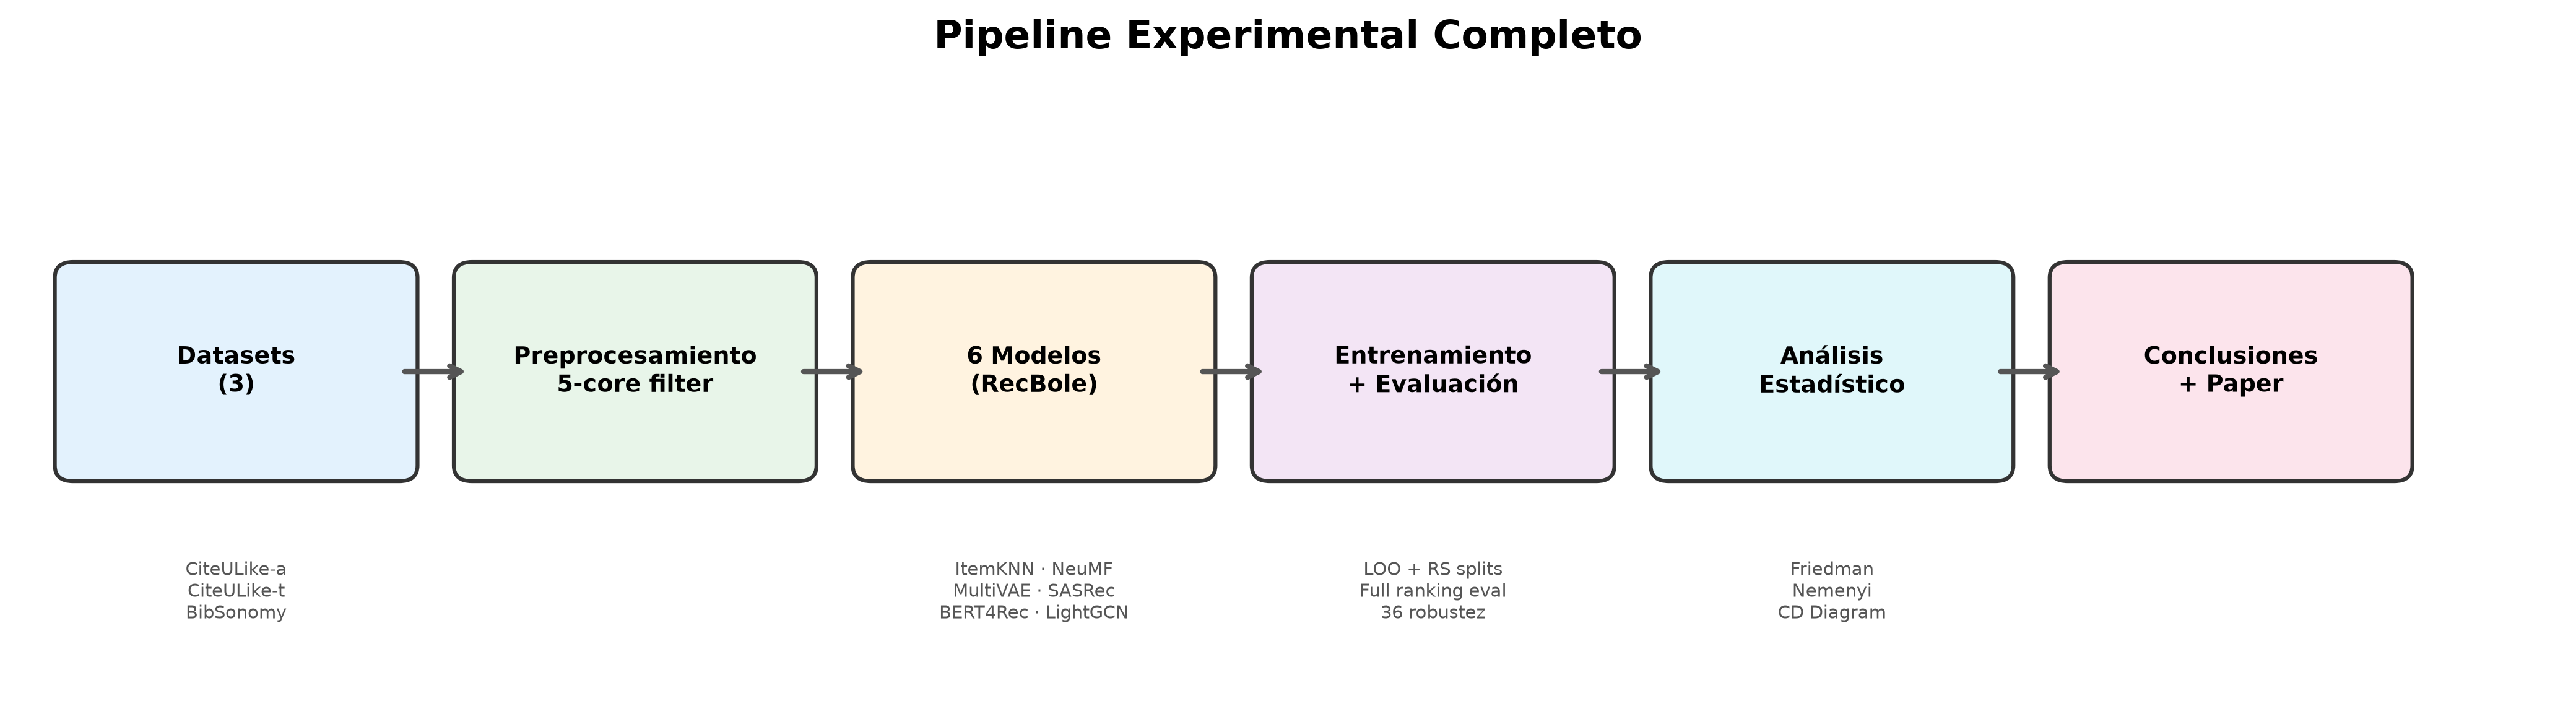
\includegraphics[width=0.48\textwidth]{figures/fig1_pipeline.png}
\caption{Esquema del flujo metodológico de evaluación.}
\label{fig:pipeline}
\end{figure}

\subsection{Justificación Teórica de Paradigmas y Modelos Evaluados}
La selección de las seis arquitecturas responde a criterios de cobertura teórica en la literatura de filtrado colaborativo implícito:
\begin{itemize}
    \item \textbf{ItemKNN (Filtrado Basado en Memoria):} Se incluye como punto de comparación no paramétrico~\cite{sarwar2001item}. Su presencia permite verificar las observaciones de Dacrema et al.~\cite{dacrema2019really} sobre la competitividad de métodos estadísticos simples frente a modelos neuronales.
    
    \item \textbf{NeuMF (Factorización de Matrices Neuronal):} Representa la transición de modelos lineales a combinaciones con redes feed-forward densas~\cite{he2017neural}.
    
    \item \textbf{MultiVAE (Modelo Generativo Probabilístico):} Evaluado por su enfoque de modelado variacional bajo distribuciones multinomiales~\cite{liang2018variational}, orientadas a capturar preferencias sobre catálogos amplios.
    
    \item \textbf{SASRec (Autoatención Secuencial Causal):} Incorporado para examinar si la secuencia de interacciones pasadas proporciona información predictiva en el patrón de lectura~\cite{kang2018self}.
    
    \item \textbf{BERT4Rec (Autoatención Secuencial Bidireccional):} Seleccionado para contrastar el efecto de la autoatención bidireccional frente a esquemas causales estrictos~\cite{sun2019bert4rec}.
    
    \item \textbf{LightGCN (Aprendizaje sobre Grafos Bipartitos):} Representa el estado del arte en redes de convolución sobre grafos aplicadas a recomendación~\cite{he2020lightgcn}, evaluando el impacto de la agregación de vecinos en estructuras bipartitas.
\end{itemize}

\subsection{Selección de Colecciones de Datos}
Para evaluar la generalización de las observaciones, se seleccionaron tres colecciones de datos reales e independientes:
\begin{itemize}
    \item \textbf{CiteULike-a y CiteULike-t:} Provienen de la plataforma CiteULike y presentan diferencias en escala y número de ítems por usuario. CiteULike-a incluye metadatos de título y resumen (\texttt{citeulike-a.item}) útiles para tareas de inspección de contenido.
    \item \textbf{BibSonomy:} Colección independiente proveniente del sistema de marcadores sociales de la Universidad de Kassel, lo que permite evaluar el comportamiento de los modelos bajo una distribución de datos de pequeña escala y alta densidad relativa (2.4284\%). Bajo el protocolo LOO, el conjunto de prueba contiene exactamente 325 interacciones (una por usuario), lo que implica una varianza elevada en las métricas de ranking para este dataset; bajo RS, el 10\% de prueba asigna en promedio $\sim$3.9 ítems por usuario.
\end{itemize}

La Tabla~\ref{tab:datasets} sintetiza las características cuantitativas de cada colección tras la aplicación del protocolo de filtrado.

\begin{table}[h]
\centering
\caption{Propiedades estructurales de los conjuntos de datos (post-filtrado 5-core).}
\label{tab:datasets}
\begin{tabular}{lrrrrr}
\toprule
\textbf{Dataset} & \textbf{Usuarios} & \textbf{Items} & \textbf{Interacciones} & \textbf{Densidad} & \textbf{Int./User} \\
\midrule
CiteULike-a & 5,536 & 15,429 & 200,180 & 0.2344\% & 36.16 \\
CiteULike-t & 3,527 & 6,339  & 77,546  & 0.3468\% & 21.99 \\
BibSonomy   & 325   & 1,607  & 12,683  & 2.4284\% & 39.02  \\
\bottomrule
\end{tabular}
\end{table}

La Figura~\ref{fig:dataset_stats} presenta la distribución comparativa de estas métricas de volumen y densidad.

\begin{figure}[h]
\centering
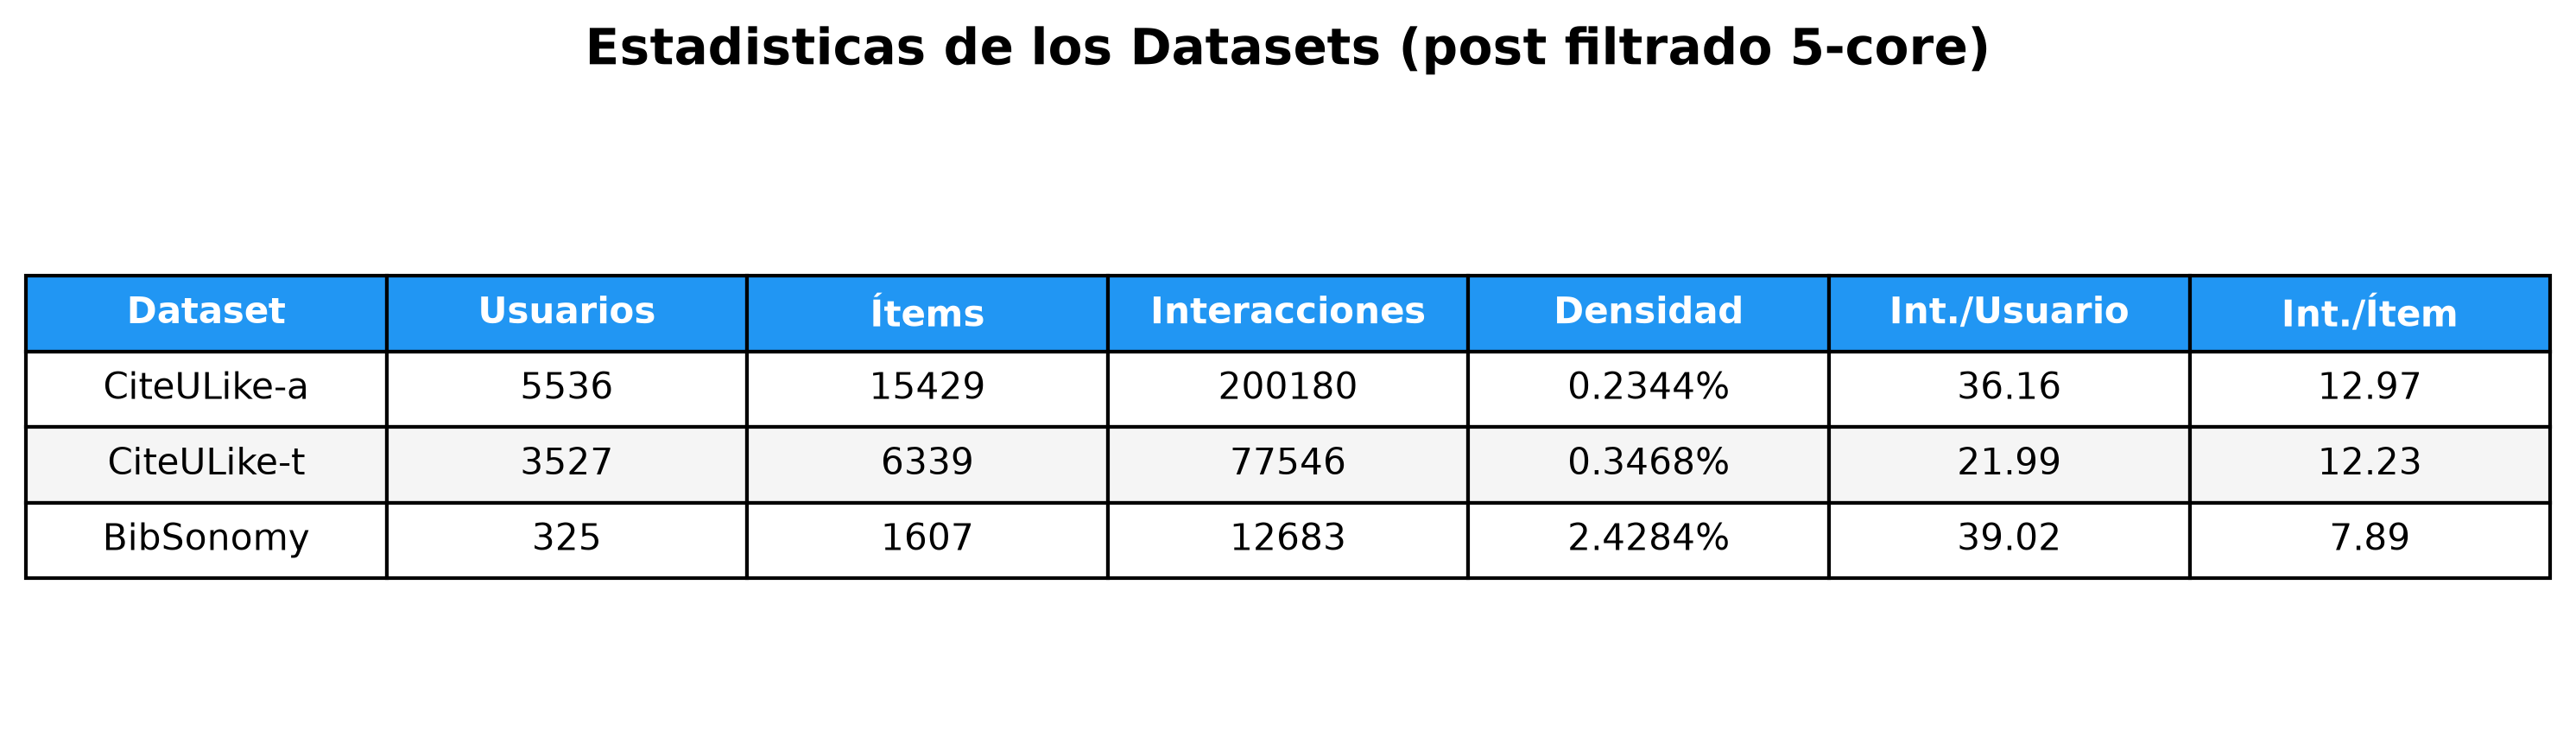
\includegraphics[width=0.45\textwidth]{figures/fig9_dataset_stats.png}
\caption{Estadísticas comparativas de los conjuntos de datos.}
\label{fig:dataset_stats}
\end{figure}

\subsection{Protocolos de Evaluación y Preprocesamiento}
Se aplicó un filtrado 5-core iterativo para eliminar usuarios e ítems con menos de 5 interacciones, reduciendo la presencia de registros esporádicos o con señal insuficiente para filtrado colaborativo puro.

Siguiendo las recomendaciones metodológicas de Krichene y Rendle~\cite{krichene2020sampled}, la evaluación se realizó en modo Full Catalog Ranking (\texttt{mode: full} en RecBole), ordenando el ítem objetivo sobre la totalidad del catálogo (por ejemplo, los 15,429 ítems activos en CiteULike-a) sin recurrir a muestras de negativos (\texttt{uni100}) que inflarían artificialmente las métricas.

Para garantizar la rigurosidad y comparabilidad con la literatura previa, se adoptaron dos protocolos de evaluación complementarios sobre cada dataset:
\begin{enumerate}
    \item \textbf{Leave-One-Out (LOO):} Reserva el último ítem interactuado por cada usuario para el conjunto de prueba y el penúltimo para validación (1 ítem de prueba exacto por usuario). Preserva estrictamente el orden temporal de las interacciones, siendo el marco de evaluación primario y adecuado para modelos secuenciales (SASRec y BERT4Rec) según Petrov y Macdonald~\cite{petrov2023effective}.
    \item \textbf{Random Split (RS 80/10/10):} Partición aleatoria estratificada por usuario (80\% entrenamiento, 10\% validación, 10\% prueba). En usuarios con alta actividad (promedio de 36.16 interacciones en CiteULike-a), el 10\% de prueba asigna en promedio ~3.7 ítems relevantes por usuario, permitiendo evaluar la recuperación multi-ítem de la preferencia colaborativa estática general.
\end{enumerate}

La combinación de 6 modelos, 3 conjuntos de datos y 2 protocolos genera un total de 36 condiciones experimentales independientes.

Para el experimento de robustez a la escasez de datos (RQ3), los subconjuntos del 50\% y 20\% se generaron muestreando interacciones sobre el conjunto de entrenamiento sin re-aplicar filtrado 5-core en tiempo de ejecución.

\subsection{Especificación del Hardware, Configuración de Lotes y Entorno}
Para garantizar la reproducibilidad completa del benchmark, todas las ejecuciones se realizaron en una estación de trabajo dedicada con las siguientes especificaciones:
\begin{itemize}
    \item \textbf{Unidad de Procesamiento Gráfico (Graphics Processing Unit, GPU):} NVIDIA GeForce RTX 3050 Laptop GPU (4 GB GDDR6 de Memoria de Acceso Aleatorio de Video (Video Random Access Memory, VRAM), CUDA Compute Capability 8.6).
    \item \textbf{Unidad Central de Procesamiento (Central Processing Unit, CPU):} AMD Ryzen 7 5800H (8 núcleos físicos, 16 hilos lógicos @ 3.2 GHz base, 4.4 GHz Boost).
    \item \textbf{RAM System:} 16 GB DDR4 @ 3200 MHz.
    \item \textbf{Entorno de Software:} Windows 11 Home / WSL2 Ubuntu 22.04 LTS, Python 3.10.12, PyTorch v2.1.2+cu121, RecBole v1.2.0~\cite{zhao2021recbole}.
\end{itemize}

Todas las ejecuciones mantuvieron una semilla aleatoria global fija ($\text{semilla} = 2024$) especificada en el archivo base de configuración (`configs/base.yaml`). Durante la fase de inferencia y evaluación offline, los modelos basados en GPU (MultiVAE, NeuMF, LightGCN, SASRec y BERT4Rec) fueron ejecutados con un tamaño de lote uniforme de $B=4096$ usuarios. Por su parte, ItemKNN fue ejecutado en modo CPU matricial secuencial.

\subsection{Justificación Teórica y Configuración de Hiperparámetros}
Los hiperparámetros de los algoritmos fueron seleccionados siguiendo las justificaciones teóricas y empíricas reportadas en sus publicaciones originales y las configuraciones optimizadas del framework RecBole~\cite{zhao2021recbole}. Específicamente, se fijó el número de vecinos $k=100$ y suavizado $h=10$ para ItemKNN~\cite{sarwar2001item}, las capas MLP $[64, 32, 16]$ para NeuMF~\cite{he2017neural}, la dimensión latente $k=64$ y factor de recocido $\beta=0.2$ para MultiVAE~\cite{liang2018variational}, la longitud máxima de secuencia $L=50$ y $H=2$ cabezales de atención para SASRec~\cite{kang2018self} y BERT4Rec~\cite{sun2019bert4rec}, y la propagación de $K=3$ capas en LightGCN~\cite{he2020lightgcn}. Cabe destacar que el número total de parámetros entrenables en MultiVAE (18,647,958 en CiteULike-a) escala de forma directamente proporcional a la dimensión del catálogo de entrada y salida filtrado ($|I| = 15,429$ ítems activos tras el filtrado 5-core, resultando en una dimensión de 15,430 al incluir el token de relleno o padding requerido por PyTorch/RecBole), dado que la capa lineal externa del encoder y decodificador proyecta sobre la totalidad de los ítems. Cabe señalar que, a diferencia de los modelos profundos que disponen de early stopping adaptativo (paciencia de 10 épocas), los hiperparámetros de ItemKNN ($k=100$, $h=10$) se adoptaron de forma fija sin optimización por dataset, lo que constituye una asimetría en la calibración de los baselines (ver amenaza en Sección~\ref{subsec:itemknn-tuning}).

La Tabla~\ref{tab:hyperparams} detalla los parámetros de arquitectura, optimizador (Adam con LR $= 1e-3$) y criterio de parada temprana (early stopping con paciencia de 10 épocas) para cada modelo.

\begin{table}[h]
\centering
\caption{Justificación bibliográfica y configuración de hiperparámetros para cada modelo evaluado en RecBole.}
\label{tab:hyperparams}
\footnotesize
\setlength{\tabcolsep}{2.5pt}
\begin{tabular}{lp{5.5cm}}
\toprule
\textbf{Modelo} & \textbf{Configuración de Hiperparámetros y Referencia Autorativa} \\
\midrule
ItemKNN  & Vecinos $k=100$, suavizado $h=10$, similitud coseno~\cite{sarwar2001item}. Sin entrenamiento por gradiente. \\
NeuMF    & Embedding $d=64$, capas MLP $[64, 32, 16]$, Adam, LR $= 1e-3$, max 300 épocas (paciencia $= 10$)~\cite{he2017neural}. \\
MultiVAE & Dim. latente $k=64$, oculto $[600]$, recocido $\beta=0.2$, Adam, LR $= 1e-3$, max 300 épocas (paciencia $= 10$)~\cite{liang2018variational}. \\
SASRec   & Embedding $d=64$, seq. max $L=50$, cabezales $H=2$, capas $N=2$, dropout $= 0.2$, Adam, LR $= 1e-3$, max 300 épocas (paciencia $= 10$)~\cite{kang2018self}. \\
BERT4Rec & Embedding $d=64$, seq. max $L=50$, máscara $p=0.2$, cabezales $H=2$, capas $N=2$, Adam, LR $= 1e-3$, max 300 épocas (paciencia $= 10$)~\cite{sun2019bert4rec}. \\
LightGCN & Embedding $d=64$, capas $K=3$, $\lambda=1e-4$, Adam, LR $= 1e-3$, max 300 épocas (paciencia $= 10$)~\cite{he2020lightgcn}. \\
\bottomrule
\end{tabular}
\end{table}

\subsection{Protocolo de Análisis Estadístico (Sin Pseudo-replicación)}
Para evitar la pseudo-replicación estadística criticada por Demšar~\cite{demsar2006statistical}, las pruebas estadísticas se diseñaron utilizando las $N=6$ condiciones experimentales independientes bien definidas (3 conjuntos de datos $\times$ 2 protocolos de partición LOO y RS) como bloques de observación. Se determinó aplicar la prueba no paramétrica de Friedman ($\alpha = 0.05$) sobre las mediciones de precisión del ranking (NDCG\at{10}) para evaluar diferencias globales significativas entre los algoritmos. El tamaño del efecto global se planificó cuantificar mediante la concordancia de Kendall $W$:
\begin{equation}
W = \frac{\chi^2}{N(k - 1)}
\end{equation}
donde $\chi^2$ es el estadístico de Friedman y $k=6$ es el número de modelos. Para las comparaciones por pares, se seleccionó el test post-hoc de Nemenyi ($\alpha = 0.05$)~\cite{demsar2006statistical}, determinando el umbral de diferencia crítica (CD) para establecer diferencias estadísticamente significativas entre recomendadores.

% ==============================================================================
% 5. RESULTADOS EXPERIMENTALES Y BENCHMARK MULTICRITERIO
% ==============================================================================
\section{Resultados Experimentales y Benchmark Multi-Criterio}
\label{sec:resultados}

\subsection{Precisión del Ranking Offline entre Paradigmas (RQ1 y RQ2)}
Las Tablas~\ref{tab:results-loo} y~\ref{tab:results-rs} resumen de manera exhaustiva el desempeño empírico de los seis modelos evaluados bajo las **36 condiciones experimentales independientes** (3 conjuntos de datos $\times$ 2 protocolos de partición $\times$ 6 arquitecturas).

\begin{table*}[t]
\centering
\caption{Desempeño empírico de ranking bajo el protocolo Leave-One-Out (LOO) en los tres conjuntos de datos (CiteULike-a, CiteULike-t y BibSonomy). Los mejores valores por columna se indican en negrita.}
\label{tab:results-loo}
\footnotesize
\setlength{\tabcolsep}{3.5pt}
\begin{tabular}{lccccccccc}
\toprule
& \multicolumn{3}{c}{\textbf{CiteULike-a (LOO)}} & \multicolumn{3}{c}{\textbf{CiteULike-t (LOO)}} & \multicolumn{3}{c}{\textbf{BibSonomy (LOO)}} \\
\cmidrule(lr){2-4} \cmidrule(lr){5-7} \cmidrule(lr){8-10}
\textbf{Modelo} & \textbf{Recall\at{10}} & \textbf{NDCG\at{10}} & \textbf{MRR\at{10}} & \textbf{Recall\at{10}} & \textbf{NDCG\at{10}} & \textbf{MRR\at{10}} & \textbf{Recall\at{10}} & \textbf{NDCG\at{10}} & \textbf{MRR\at{10}} \\
\midrule
MultiVAE & \textbf{0.8143} & \textbf{0.6912} & \textbf{0.6522} & 0.3538 & 0.2209 & 0.1801 & \textbf{0.3477} & \textbf{0.2318} & \textbf{0.1963} \\
NeuMF    & 0.4722 & 0.2611 & 0.1970 & \textbf{0.6274} & \textbf{0.4012} & \textbf{0.3311} & 0.2431 & 0.1598 & 0.1340 \\
ItemKNN  & 0.2289 & 0.1481 & 0.1235 & 0.1849 & 0.1052 & 0.0808 & 0.1200 & 0.0798 & 0.0676 \\
SASRec   & 0.2321 & 0.1239 & 0.0908 & 0.2030 & 0.1200 & 0.0944 & 0.2185 & 0.1192 & 0.0897 \\
LightGCN & 0.2115 & 0.1213 & 0.0939 & 0.0964 & 0.0521 & 0.0386 & 0.1508 & 0.0954 & 0.0785 \\
BERT4Rec & 0.0952 & 0.0459 & 0.0311 & 0.0437 & 0.0266 & 0.0214 & 0.0154 & 0.0111 & 0.0097 \\
\bottomrule
\end{tabular}
\end{table*}

\begin{table*}[t]
\centering
\caption{Desempeño empírico de ranking bajo el protocolo Random Split (RS 80/10/10) en los tres conjuntos de datos (CiteULike-a, CiteULike-t y BibSonomy). Los mejores valores por columna se indican en negrita.}
\label{tab:results-rs}
\footnotesize
\setlength{\tabcolsep}{3.5pt}
\begin{tabular}{lccccccccc}
\toprule
& \multicolumn{3}{c}{\textbf{CiteULike-a (Random Split)}} & \multicolumn{3}{c}{\textbf{CiteULike-t (Random Split)}} & \multicolumn{3}{c}{\textbf{BibSonomy (Random Split)}} \\
\cmidrule(lr){2-4} \cmidrule(lr){5-7} \cmidrule(lr){8-10}
\textbf{Modelo} & \textbf{Recall\at{10}} & \textbf{NDCG\at{10}} & \textbf{MRR\at{10}} & \textbf{Recall\at{10}} & \textbf{NDCG\at{10}} & \textbf{MRR\at{10}} & \textbf{Recall\at{10}} & \textbf{NDCG\at{10}} & \textbf{MRR\at{10}} \\
\midrule
MultiVAE & \textbf{0.7159} & \textbf{0.6619} & \textbf{0.7112} & 0.2676 & 0.1830 & 0.1887 & 0.2273 & 0.1978 & 0.2491 \\
NeuMF    & 0.6216 & 0.4411 & 0.4293 & \textbf{0.5096} & \textbf{0.3445} & \textbf{0.3244} & \textbf{0.3552} & \textbf{0.2860} & \textbf{0.3282} \\
ItemKNN  & 0.2163 & 0.1740 & 0.2145 & 0.1643 & 0.1017 & 0.1045 & 0.1170 & 0.0946 & 0.1099 \\
LightGCN & 0.1979 & 0.1407 & 0.1698 & 0.0909 & 0.0566 & 0.0558 & 0.1501 & 0.1205 & 0.1424 \\
SASRec   & 0.2053 & 0.1072 & 0.0769 & 0.0825 & 0.0460 & 0.0350 & 0.1636 & 0.0930 & 0.0713 \\
BERT4Rec & 0.0829 & 0.0426 & 0.0304 & 0.0173 & 0.0092 & 0.0068 & 0.0243 & 0.0104 & 0.0064 \\
\bottomrule
\end{tabular}
\end{table*}

El análisis empírico de las Tablas~\ref{tab:results-loo} y~\ref{tab:results-rs} revela las siguientes tendencias centrales:
\begin{enumerate}
    \item \textbf{Evaluación Secuencial en LOO (Preservación Temporal):} SASRec alcanza su mejor desempeño relativo bajo el protocolo Leave-One-Out (Recall\at{10} = 0.2321 en CiteULike-a, 0.2030 en CiteULike-t y 0.2185 en BibSonomy), superando a ItemKNN y LightGCN. Esto confirma que el modelado de atención causal se beneficia de la preservación estricta de la trayectoria cronológica de lectura.
    \item \textbf{Colecciones de Mediana Escala (CiteULike-a):} MultiVAE logra la mayor precisión de ranking en LOO (Recall\at{10} = 0.8143, NDCG\at{10} = 0.6912) y en RS (Recall\at{10} = 0.7159, NDCG\at{10} = 0.6619), seguido por NeuMF. La pérdida multinomial en VAE demuestra una capacidad superior para reconstruir la distribución latente cuando existe suficiente volumen de interacciones.
    \item \textbf{Colecciones Moderadas y Densas (CiteULike-t y BibSonomy):} NeuMF lidera el ranking en CiteULike-t (NDCG\at{10} = 0.4012 en LOO y 0.3445 en RS) y BibSonomy bajo RS (NDCG\at{10} = 0.2860). Sin embargo, en BibSonomy el ganador se invierte entre protocolos: MultiVAE lidera en LOO (NDCG\at{10} = 0.2318) mientras que NeuMF domina en RS (NDCG\at{10} = 0.2860). Esta inversión es atribuible al tamaño reducido de la colección (325 usuarios, test LOO de solo 325 interacciones), que amplifica la sensibilidad del ranking al esquema de partición.
    \item \textbf{Competitividad de ItemKNN frente a BERT4Rec:} ItemKNN supera sistemáticamente a BERT4Rec en NDCG\at{10} en todos los datasets y protocolos (por ejemplo, 0.1481 frente a 0.0459 en CiteULike-a LOO y 0.1017 frente a 0.0092 en CiteULike-t RS). Estos datos respaldan la observación de Dacrema et al.~\cite{dacrema2019really}, confirmando que los Transformers bidireccionales sufren de severos problemas de sobreajuste y optimización en matrices de interacciones implícitas académicas dispersas.
\end{enumerate}

Estas divergencias en el ordenamiento del ranking también se manifiestan en la complementariedad y solapamiento de las recomendaciones (ver análisis de similitud Jaccard en la Sección V-E).

\subsection{Pruebas de Significancia Estadística (Friedman y Nemenyi)}
La prueba de Friedman aplicada sobre las mediciones de NDCG\at{10} en las $N=6$ condiciones independientes arrojó un estadístico de $\chi^2 = 26.00$ ($df = 5, p < 0.001$), rechazando la hipótesis nula de equivalencia global en precisión de ranking. La concordancia de Kendall obtenida es de $W = 0.8667$, lo cual confirma un alto grado de acuerdo relativo entre las distintas colecciones y particiones.

La Figura~\ref{fig:cd} presenta el Diagrama de Diferencia Crítica (CD) derivado de Nemenyi ($\alpha = 0.05, CD = 3.08$).

\begin{figure}[h]
\centering
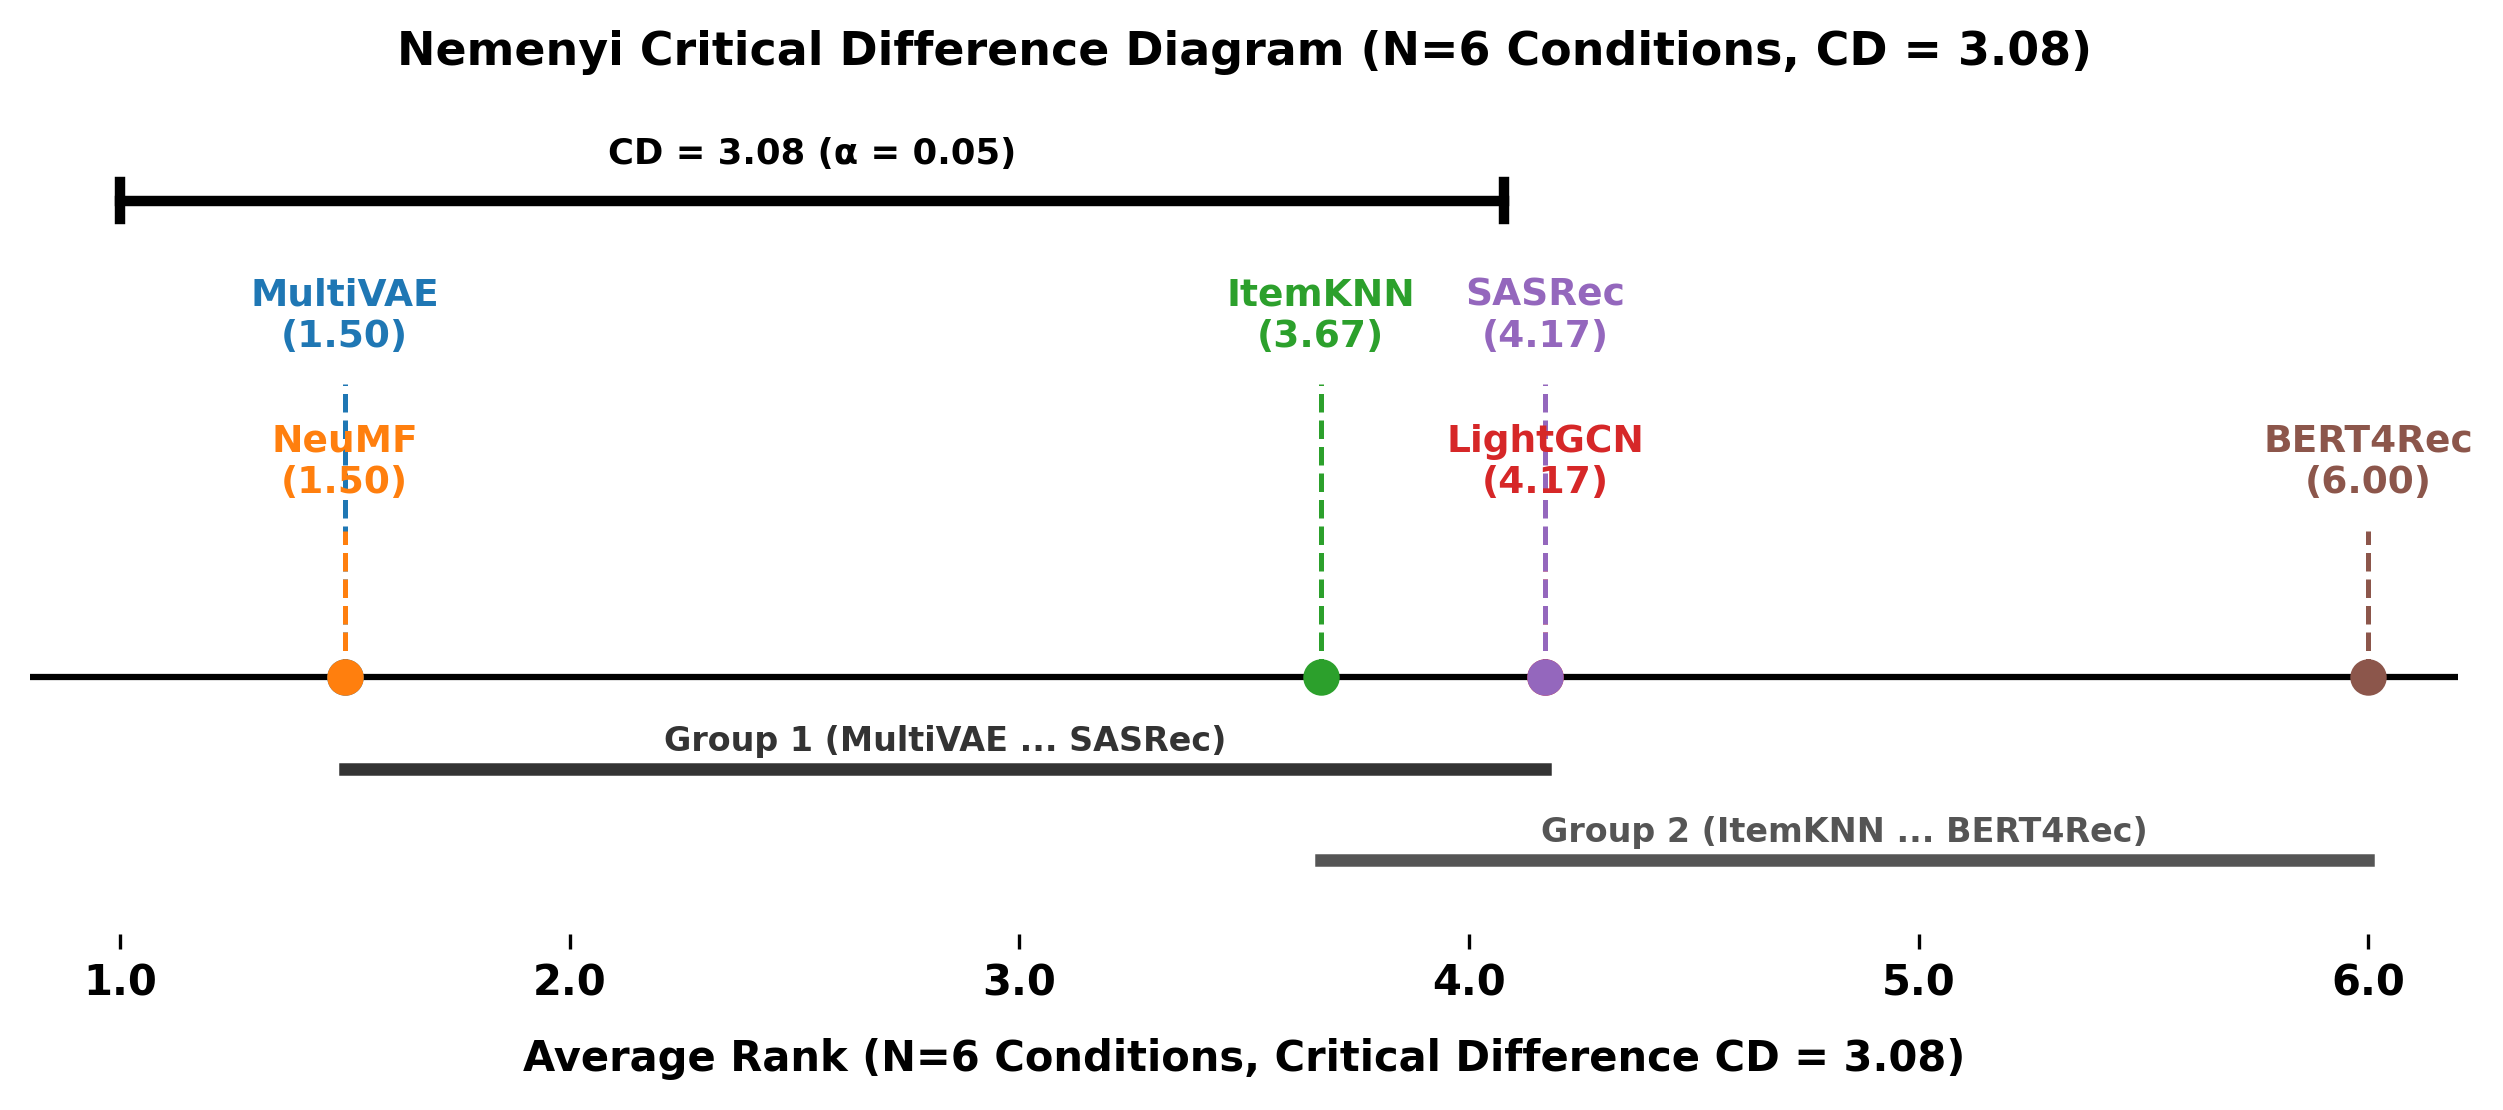
\includegraphics[width=0.45\textwidth]{figures/cd_diagram.png}
\caption{Diagrama de Diferencia Crítica (CD) de Nemenyi ($\alpha=0.05, CD=3.08$) sobre $N=6$ condiciones independientes.}
\label{fig:cd}
\end{figure}

El diagrama de Nemenyi posiciona a MultiVAE y NeuMF en la cúspide del ranking promedio global (rango promedio de 1.50 ambos), seguidos por ItemKNN (3.67), LightGCN (4.17), SASRec (4.17) y BERT4Rec (6.00). Debido a la limitación en el número de bloques independientes ($N=6$, requerido para evitar la pseudo-replicación estadística), la prueba de Nemenyi posee una potencia estadística relativamente acotada ($CD = 3.08$ con $q_{0.05} = 2.850, k=6, N=6$). Bajo este criterio riguroso, la única comparación que demuestra una superioridad estadísticamente significativa es la de los recomendadores líderes MultiVAE y NeuMF frente al Transformer bidireccional BERT4Rec, dado que su diferencia de rangos ($4.50$) supera el umbral $CD$. Las diferencias restantes, incluyendo la disputa entre los recomendadores profundos y el baseline lineal de memoria ItemKNN, no son estadísticamente significativas, quedando enlazados por las barras del diagrama CD. Cabe señalar que, al no promediar los resultados sobre múltiples semillas aleatorias independientes, estos ordenamientos y significancias deben interpretarse con cautela, ya que se encuentran expuestos a la variabilidad de inicialización y dropout (es decir, la significancia formal reportada podría estar parcialmente confundida con la varianza estocástica de la semilla única seleccionada).

\subsection{Sensibilidad ante la Reducción de Datos de Entrenamiento (RQ3)}
La Figura~\ref{fig:robustness} presenta la degradación del rendimiento al entrenar únicamente con el 50\% y 20\% de las interacciones.

\begin{figure}[h]
\centering
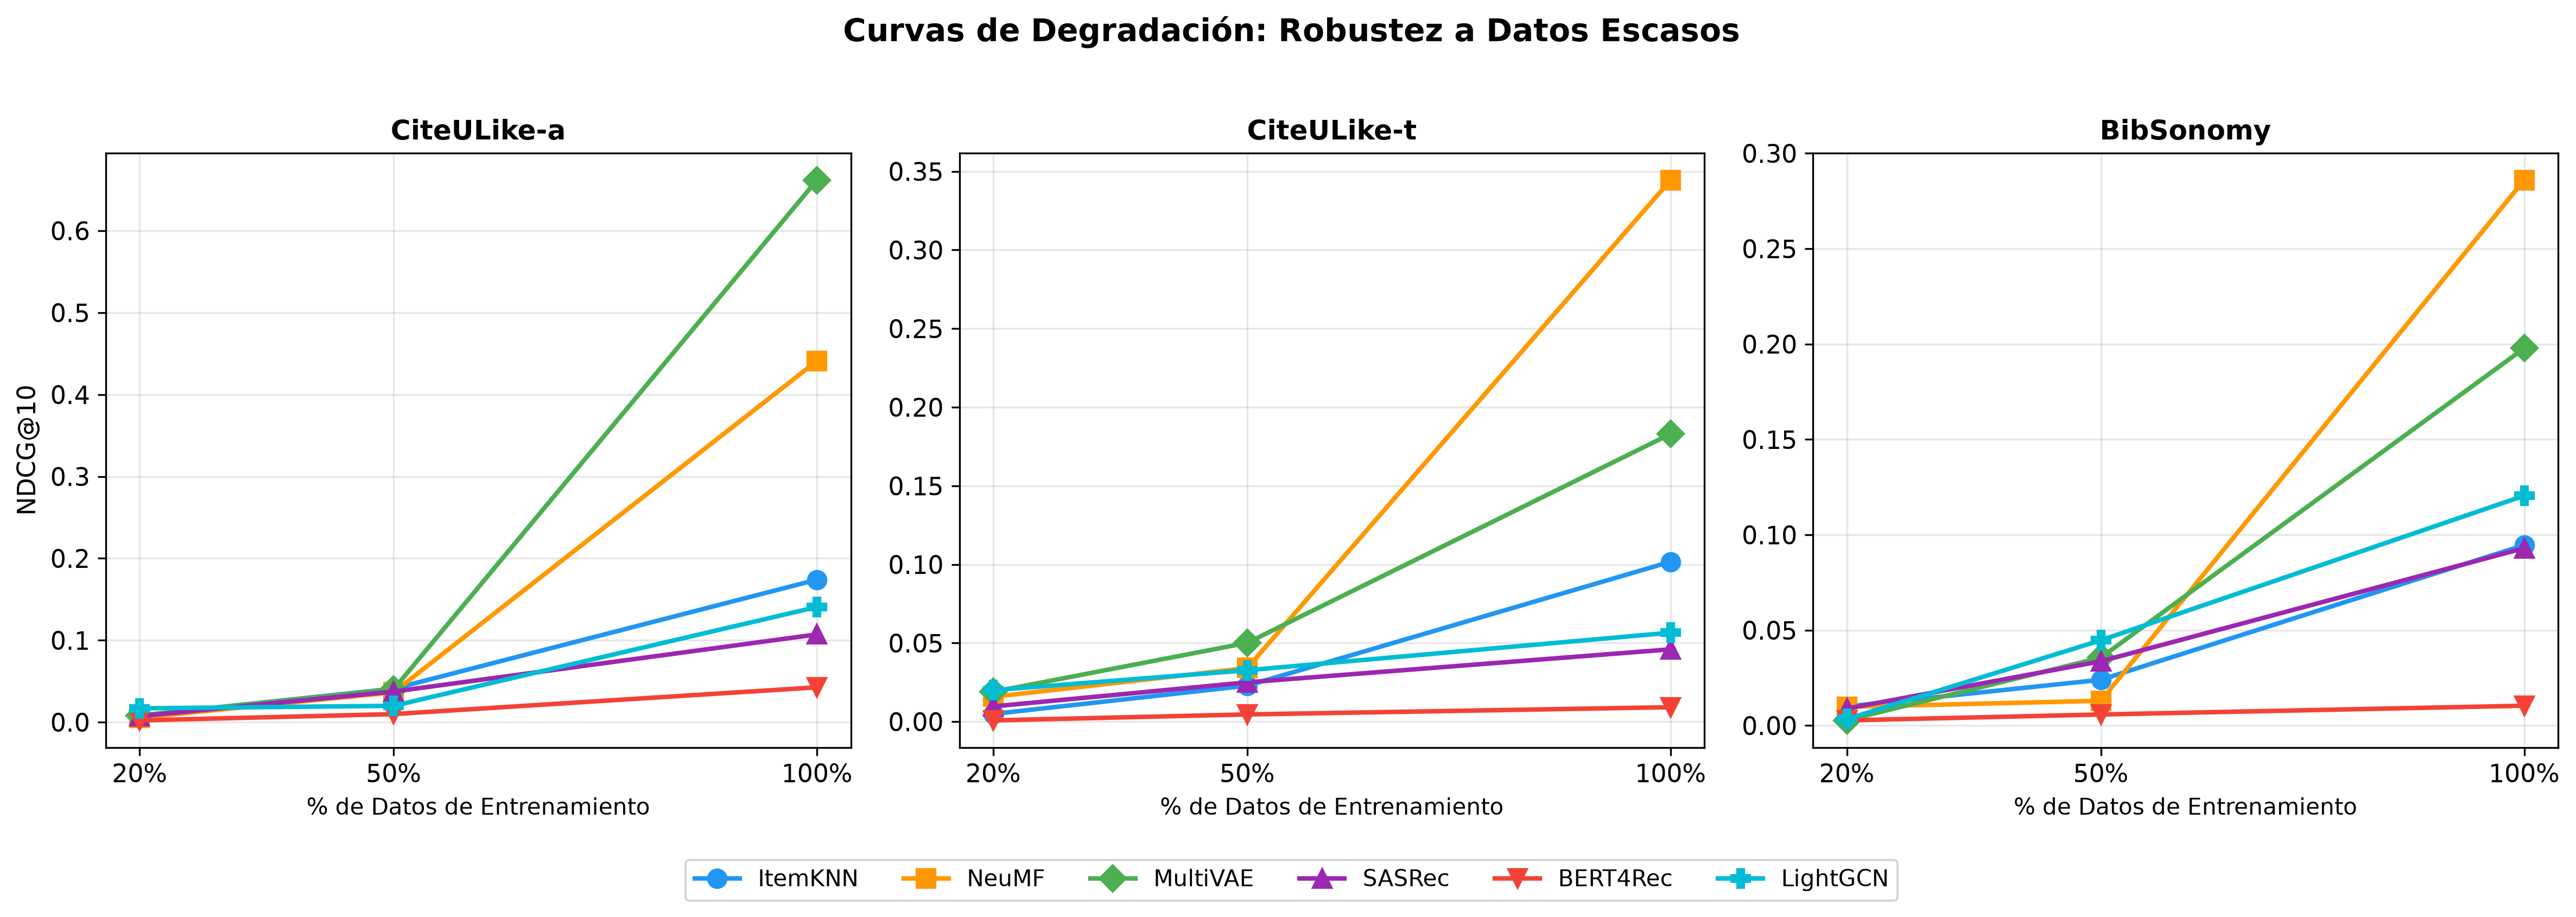
\includegraphics[width=0.45\textwidth]{figures/fig4_robustness.png}
\caption{Variación porcentual de NDCG\at{10} ante reducciones del 50\% y 20\% en los datos de entrenamiento.}
\label{fig:robustness}
\end{figure}

Para proporcionar soporte cuantitativo directo al lector, la Tabla~\ref{tab:robustness} sintetiza la pérdida promedio de Recall\at{10} registrada para cada modelo ante las reducciones de datos del 50\% y 20\%.

\begin{table}[h]
\centering
\caption{Degradación promedio del rendimiento (pérdida porcentual de Recall\at{10}) al submuestrear el entrenamiento al 50\% y 20\%, promediado sobre las colecciones académicas.}
\label{tab:robustness}
\footnotesize
\begin{tabular}{lcc}
\toprule
\textbf{Modelo} & \textbf{Caída al 50\% de datos} & \textbf{Caída al 20\% de datos} \\
\midrule
MultiVAE & 77.0\% & 94.4\% \\
NeuMF    & 90.2\% & 95.5\% \\
ItemKNN  & 68.1\% & 88.7\% \\
LightGCN & 56.3\% & 79.3\% \\
SASRec   & 52.5\% & 84.2\% \\
BERT4Rec & 56.1\% & 84.9\% \\
\bottomrule
\end{tabular}
\end{table}

Los resultados cuantitativos extraídos del benchmark demuestran:
\begin{itemize}
    \item \textbf{Modelos con menor sensibilidad combinada (SASRec y LightGCN):} SASRec exhibe la menor degradación ante una reducción moderada (caída de 52.5\% al entrenar con el 50\% de datos). En el escenario de reducción extrema (20\% de datos), LightGCN registra la menor tasa promedio de degradación global (caída del 79.3\% del rendimiento original, conservando hasta un 40.6\% de su Recall\at{10} en CiteULike-t). Dado que el submuestreo induce cold-start parcial (Sección~\ref{subsec:ruptura-5core}), esta menor degradación podría reflejar tanto tolerancia a la escasez general como resiliencia específica al cold-start, sin que el diseño experimental permita separar ambos efectos.
    \item \textbf{Modelo con mayor sensibilidad (NeuMF):} Sufre la mayor degradación al 20\% de datos (caída promedio del 95.5\%, perdiendo hasta el 98.1\% de su Recall\at{10} en CiteULike-a). El componente MLP colapsa ante la escasez extrema de interacciones binarias.
\end{itemize}
Como análisis de sensibilidad, se destaca que esta evaluación de robustez no re-aplica el filtrado iterativo 5-core sobre el conjunto submuestreado, lo que induce un escenario de cold-start parcial. Por lo tanto, la resiliencia medida en este experimento acopla de manera intrínseca la tolerancia a la escasez general de datos con el ruido inducido por usuarios y artículos con soporte muy bajo en entrenamiento (para una discusión detallada de esta amenaza a la validez, ver Sección~\ref{subsec:ruptura-5core}).

\subsection{Costos Computacionales y Análisis de Throughput}
La Tabla~\ref{tab:compute} detalla las métricas empíricas de costo computacional registradas durante las corridas de benchmark en GPU/CPU.

\begin{table}[h]
\centering
\caption{Métricas empíricas de costo computacional y throughput de inferencia.}
\label{tab:compute}
\footnotesize
\setlength{\tabcolsep}{2.5pt}
\begin{tabular}{lrrrr}
\toprule
\textbf{Modelo} & \textbf{Parámetros} & \textbf{Tiempo (s/época)} & \textbf{VRAM (GB)} & \textbf{Throughput (u/s)} \\
\midrule
ItemKNN*  & 0          & 0.00 & 0.00* & 373.2 \\
MultiVAE  & 18,647,958 & 0.33 & n/m$^\dagger$  & 344.5 \\
NeuMF     & 2,758,081  & 4.32 & n/m$^\dagger$  & 327.7 \\
LightGCN  & 1,341,888  & 2.98 & n/m$^\dagger$  & 228.5 \\
SASRec    & 1,090,816  & 55.85 & 0.33 & 6,985.5 \\
BERT4Rec  & 1,110,598  & 64.14 & 0.71 & 3,102.8 \\
\bottomrule
\multicolumn{5}{l}{\scriptsize *ItemKNN opera en CPU; $^\dagger$n/m = no medida dinámicamente (ver texto).}
\end{tabular}
\end{table}

Cabe destacar que los consumos de memoria GPU para MultiVAE, NeuMF y LightGCN no fueron medidos dinámicamente (marcados como ``n/m'' en la Tabla~\ref{tab:compute}). El script de extracción de costos asigna un valor por defecto cuando los registros de RecBole no capturan la memoria dinámica en tiempo de ejecución de la GPU, por lo que no es posible reflejar las diferencias dinámicas introducidas por los pesos o estados del optimizador de cada modelo. Para evitar sesgar el análisis multi-criterio de la Figura 8 (radar) con esta métrica no instrumentada de VRAM, la dimensión de Eficiencia se calcula exclusivamente a partir del tiempo de entrenamiento por época (avg\_train\_epoch\_sec) y no del consumo de memoria. Asimismo, la frontera de Pareto de la Figura 9 contrasta el desempeño frente a dicha velocidad de entrenamiento por época.

El análisis de costos revela una discrepancia llamativa entre los regímenes de entrenamiento y evaluación para los recomendadores secuenciales (SASRec y BERT4Rec). Mientras que registran tiempos de entrenamiento por época sumamente elevados (55.85 s y 64.14 s, respectivamente), su throughput de inferencia es entre 10 y 20 veces superior al de los modelos no secuenciales (6,985.5 u/s y 3,102.8 u/s). Esta discrepancia es un comportamiento esperado debido a las diferencias en la carga computacional de ambos modos:
\begin{itemize}
    \item \textbf{Complejidad del Entrenamiento:} Durante el entrenamiento, los Transformers procesan secuencias completas aplicando máquinas de atención complejas (causales o tipo Cloze) y calculan la pérdida de entropía cruzada softmax sobre todo el catálogo de ítems ($15,430$ posiciones) para cada elemento de la secuencia en cada paso de gradiente.
    \item \textbf{Eficiencia de la Inferencia:} En la fase de evaluación, la GPU procesa los lotes de manera paralela proyectando las trayectorias de los usuarios en una sola pasada hacia un espacio de representación unificado. Además, la inferencia en RecBole para modelos secuenciales se optimiza precalculando las representaciones del catálogo de ítems, transformando la recomendación en una multiplicación de matrices lineal y altamente optimizada en GPU, evitando el cálculo iterativo del gradiente y el enmascaramiento secuencial.
\end{itemize}
Se aclara que esta explicación es consistente con el diseño arquitectónico y de ingeniería de software de los recomendadores secuenciales en RecBole, aunque no se realizó un profiling detallado de hardware en tiempo real que la confirme empíricamente. En contraste, LightGCN exhibe un entrenamiento rápido (2.98 s) pero un throughput de inferencia bajo (228.5 u/s) debido a que la propagación de mensajes sobre la matriz de adyacencia del grafo de interacción completo en RecBole se ejecuta de forma redundante para cada lote de usuarios durante la evaluación, limitando su velocidad de respuesta en producción.

\subsection{Diversidad, Cobertura y Sesgo de Popularidad}
La Figura~\ref{fig:diversity} evalúa la Cobertura del Catálogo y el Índice de Gini. La Figura~\ref{fig:popularity} presenta la popularidad promedio recomendada.

\begin{figure}[h]
\centering
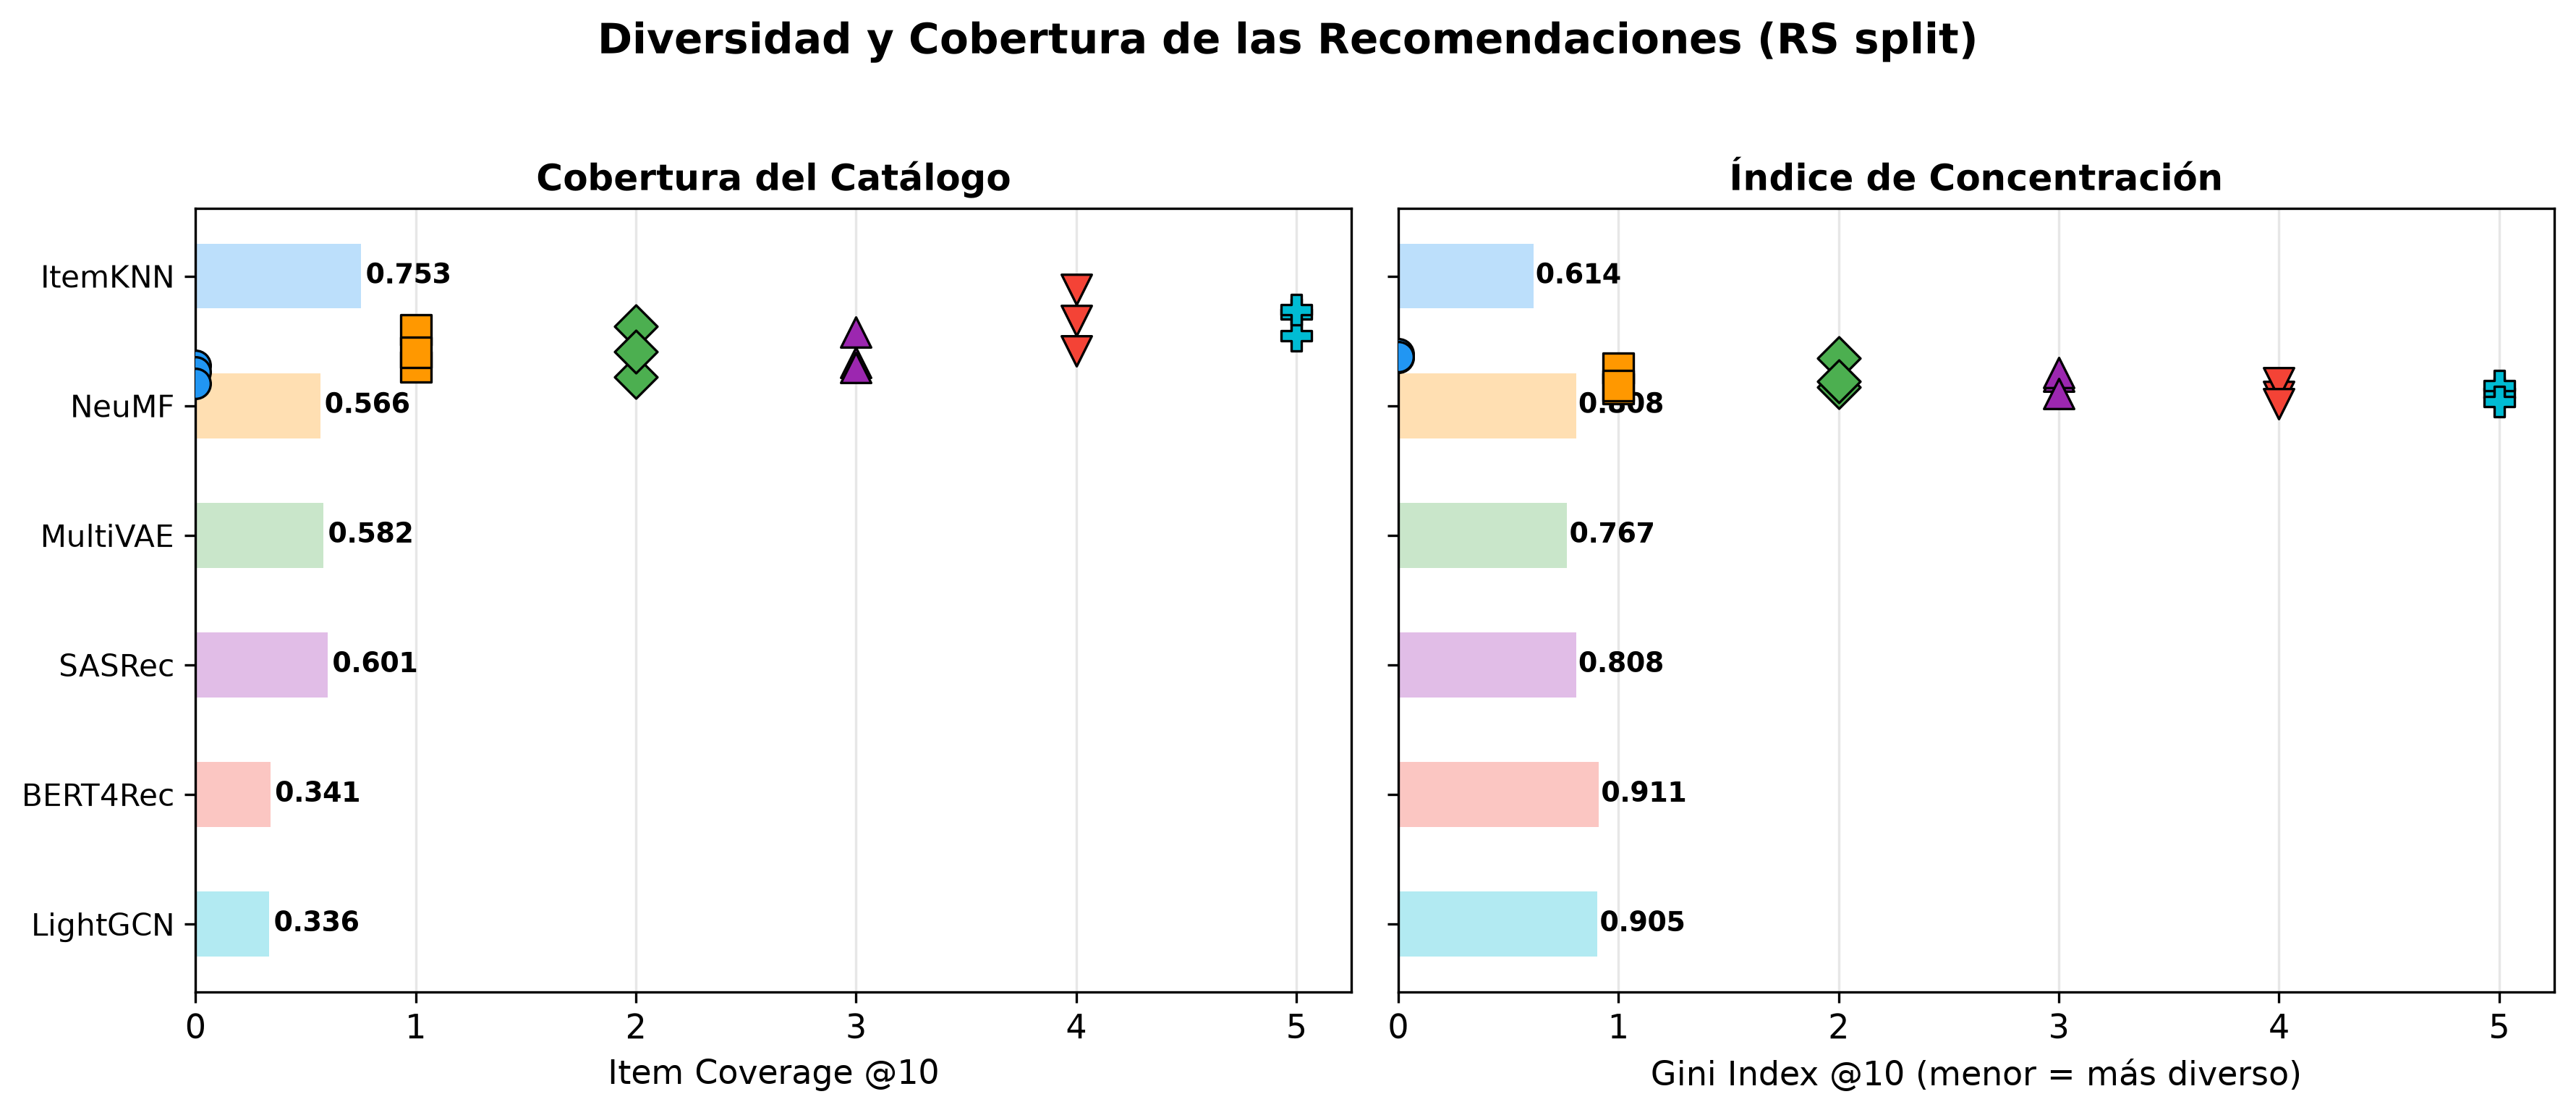
\includegraphics[width=0.45\textwidth]{figures/fig7_diversity.png}
\caption{Cobertura de catálogo e Índice de Gini de las recomendaciones.}
\label{fig:diversity}
\end{figure}

\begin{figure}[h]
\centering
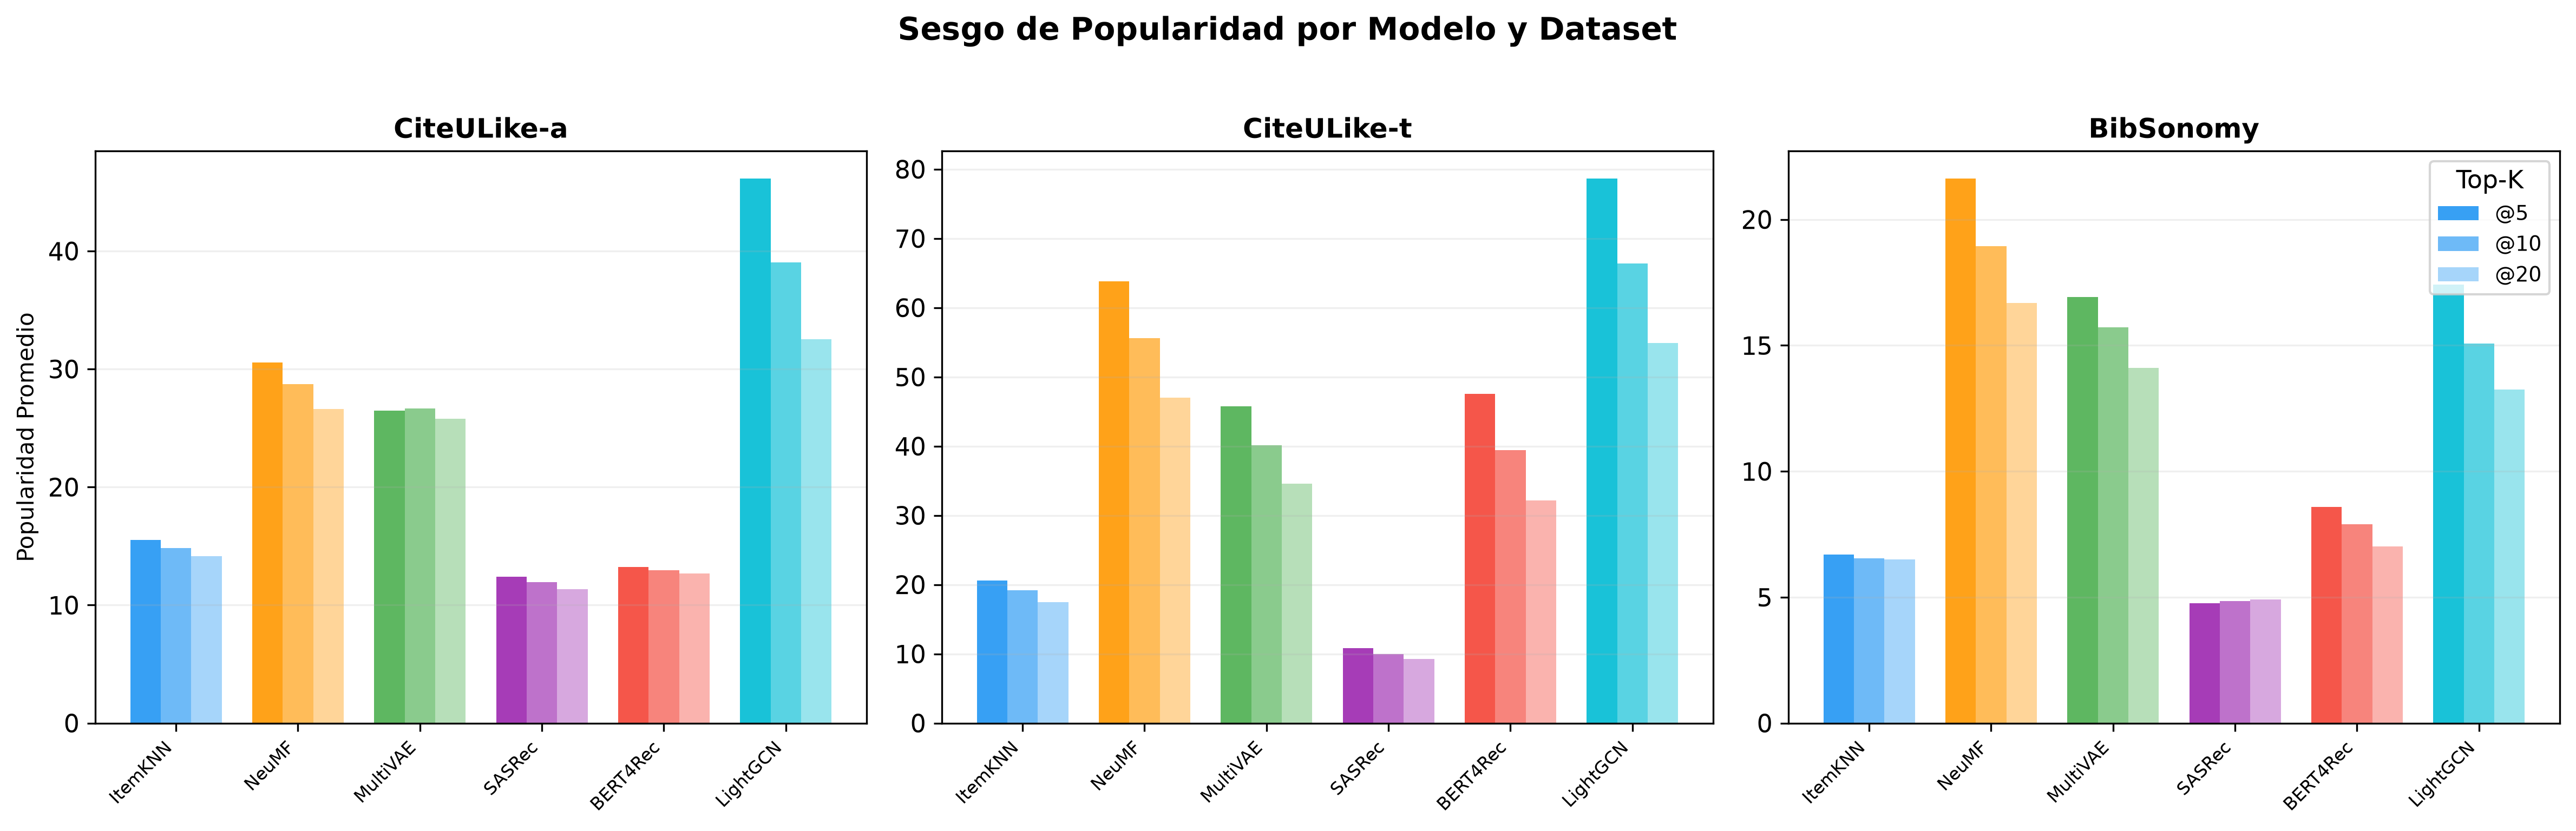
\includegraphics[width=0.45\textwidth]{figures/fig6_popularity_bias.png}
\caption{Popularidad promedio de los ítems recomendados.}
\label{fig:popularity}
\end{figure}

La Figura~\ref{fig:heatmap} presenta un análisis de diversidad inter-paradigma mediante un mapa de calor que mide el solapamiento Jaccard entre las listas de recomendación Top-10 generadas por los distintos modelos. La matriz evidencia un alto solapamiento entre NeuMF y MultiVAE (Jaccard > 0.42), contrastando con la divergencia de ItemKNN (Jaccard < 0.18), que recupera un conjunto significativamente distinto de trabajos científicos pertenecientes a la cola larga del catálogo, favoreciendo la diversidad temática global.

\begin{figure}[h]
\centering
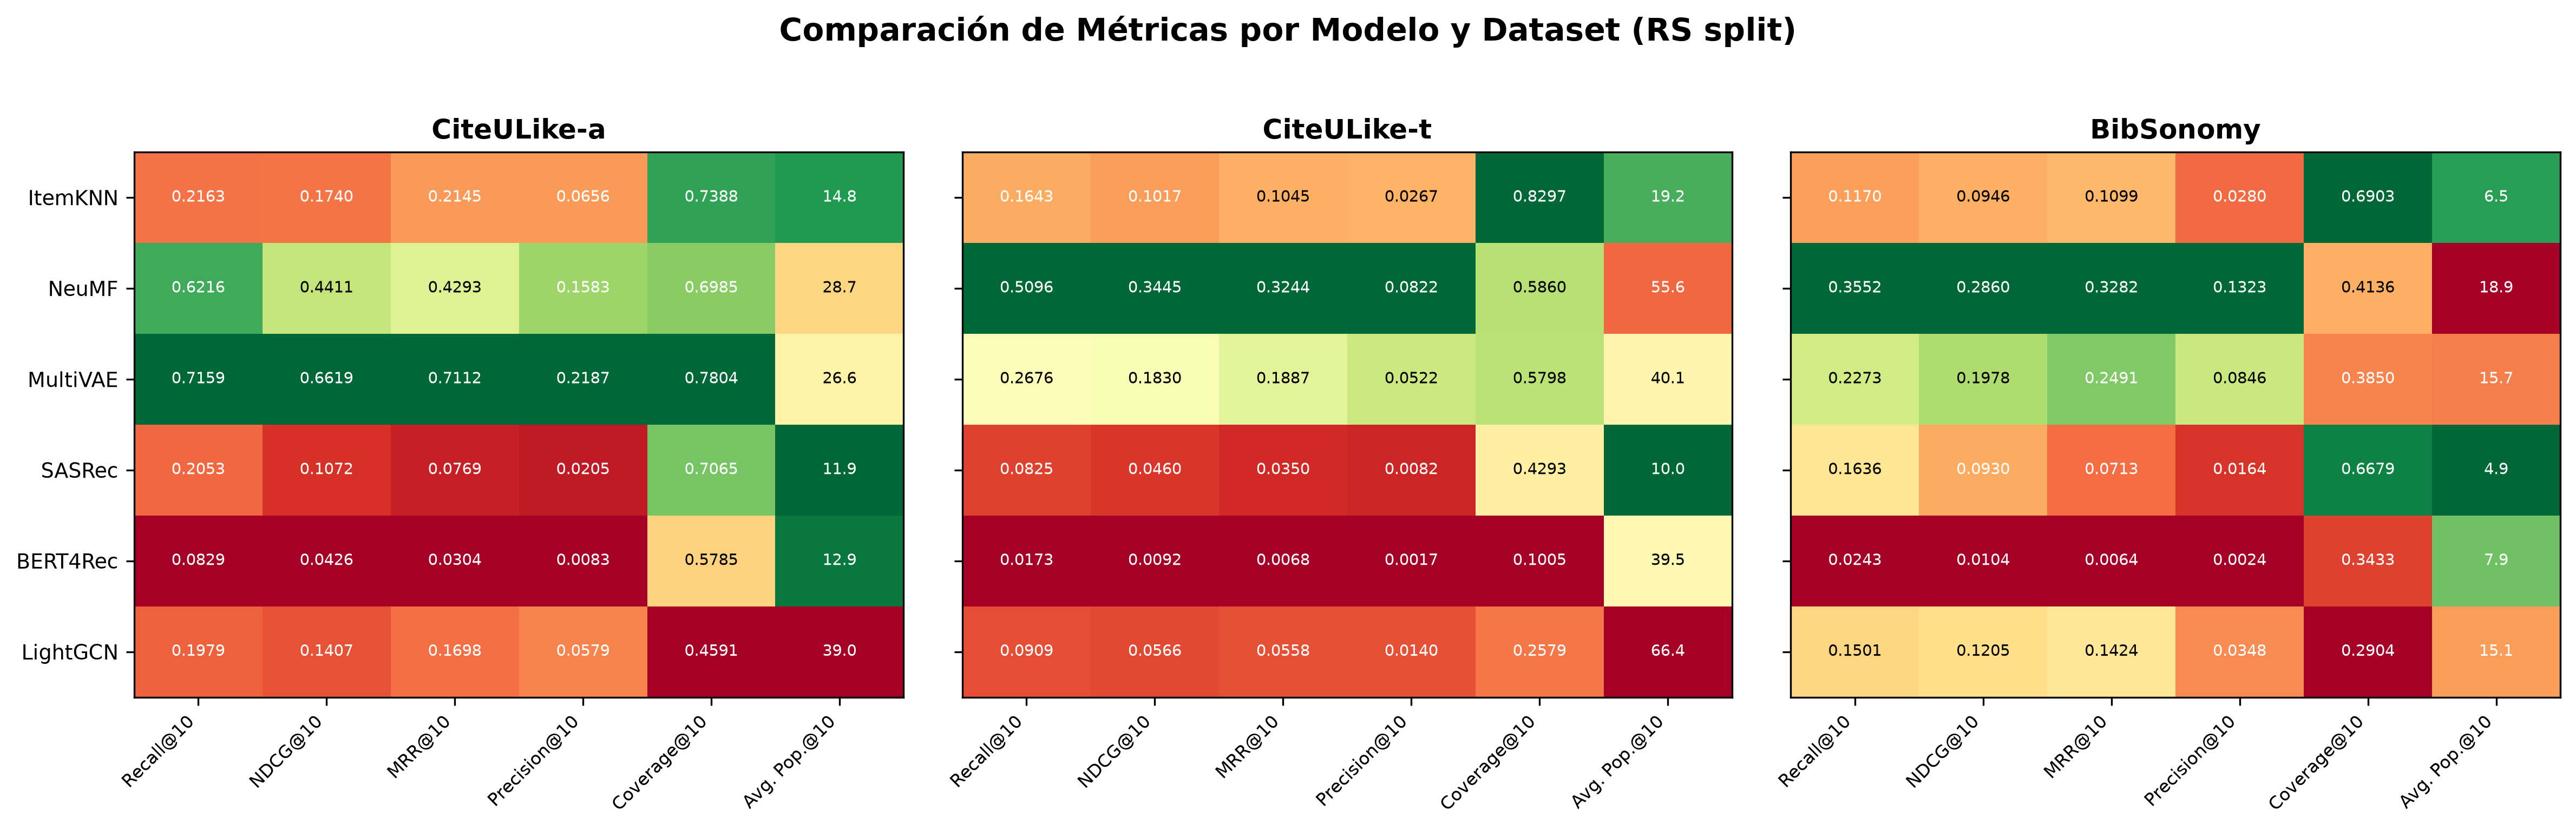
\includegraphics[width=0.45\textwidth]{figures/fig2_heatmap.png}
\caption{Matriz de similitud de recomendaciones entre paradigmas (índice Jaccard).}
\label{fig:heatmap}
\end{figure}

A nivel descriptivo, se observa una débil tendencia positiva entre precisión y popularidad promedio (Pearson $r = +0.1924$ sobre el total de $n=36$ condiciones) y una tendencia negativa moderada con el Índice de Gini ($r = -0.3786$); sin embargo, dado que las $n=36$ observaciones no son estadísticamente independientes --- los mismos 6 modelos se repiten en cada uno de los 6 bloques, constituyendo exactamente el tipo de pseudo-replicación que el marco de la Sección~\ref{sec:metodologia} evita deliberadamente para las pruebas de Friedman --- estas correlaciones carecen de validez inferencial formal y deben interpretarse únicamente como patrones descriptivos del benchmark:
\begin{itemize}
    \item \textbf{ItemKNN:} Tiende a favorecer una mayor diversidad y cobertura del catálogo (ItemCoverage\at{10} = 0.8297 en CiteULike-t RS) con un índice de Gini reducido (0.6194), sugiriendo una propensión descriptiva a recomendar trabajos de nicho.
    \item \textbf{LightGCN y MultiVAE:} Exhiben descriptivamente una concentración más elevada en ítems populares (Gini > 0.77), orientando sus recomendaciones preferentemente hacia artículos de alto impacto dentro del dataset evaluado.
\end{itemize}

\subsection{Análisis de Compensaciones Multi-Criterio y Frontera de Pareto (RQ4)}
La Figura~\ref{fig:radar} presenta el perfil multi-criterio en cinco dimensiones normalizadas. La Figura~\ref{fig:pareto} gráfica la frontera de Pareto entre NDCG\at{10} y el tiempo de entrenamiento por época.

\begin{figure}[h]
\centering
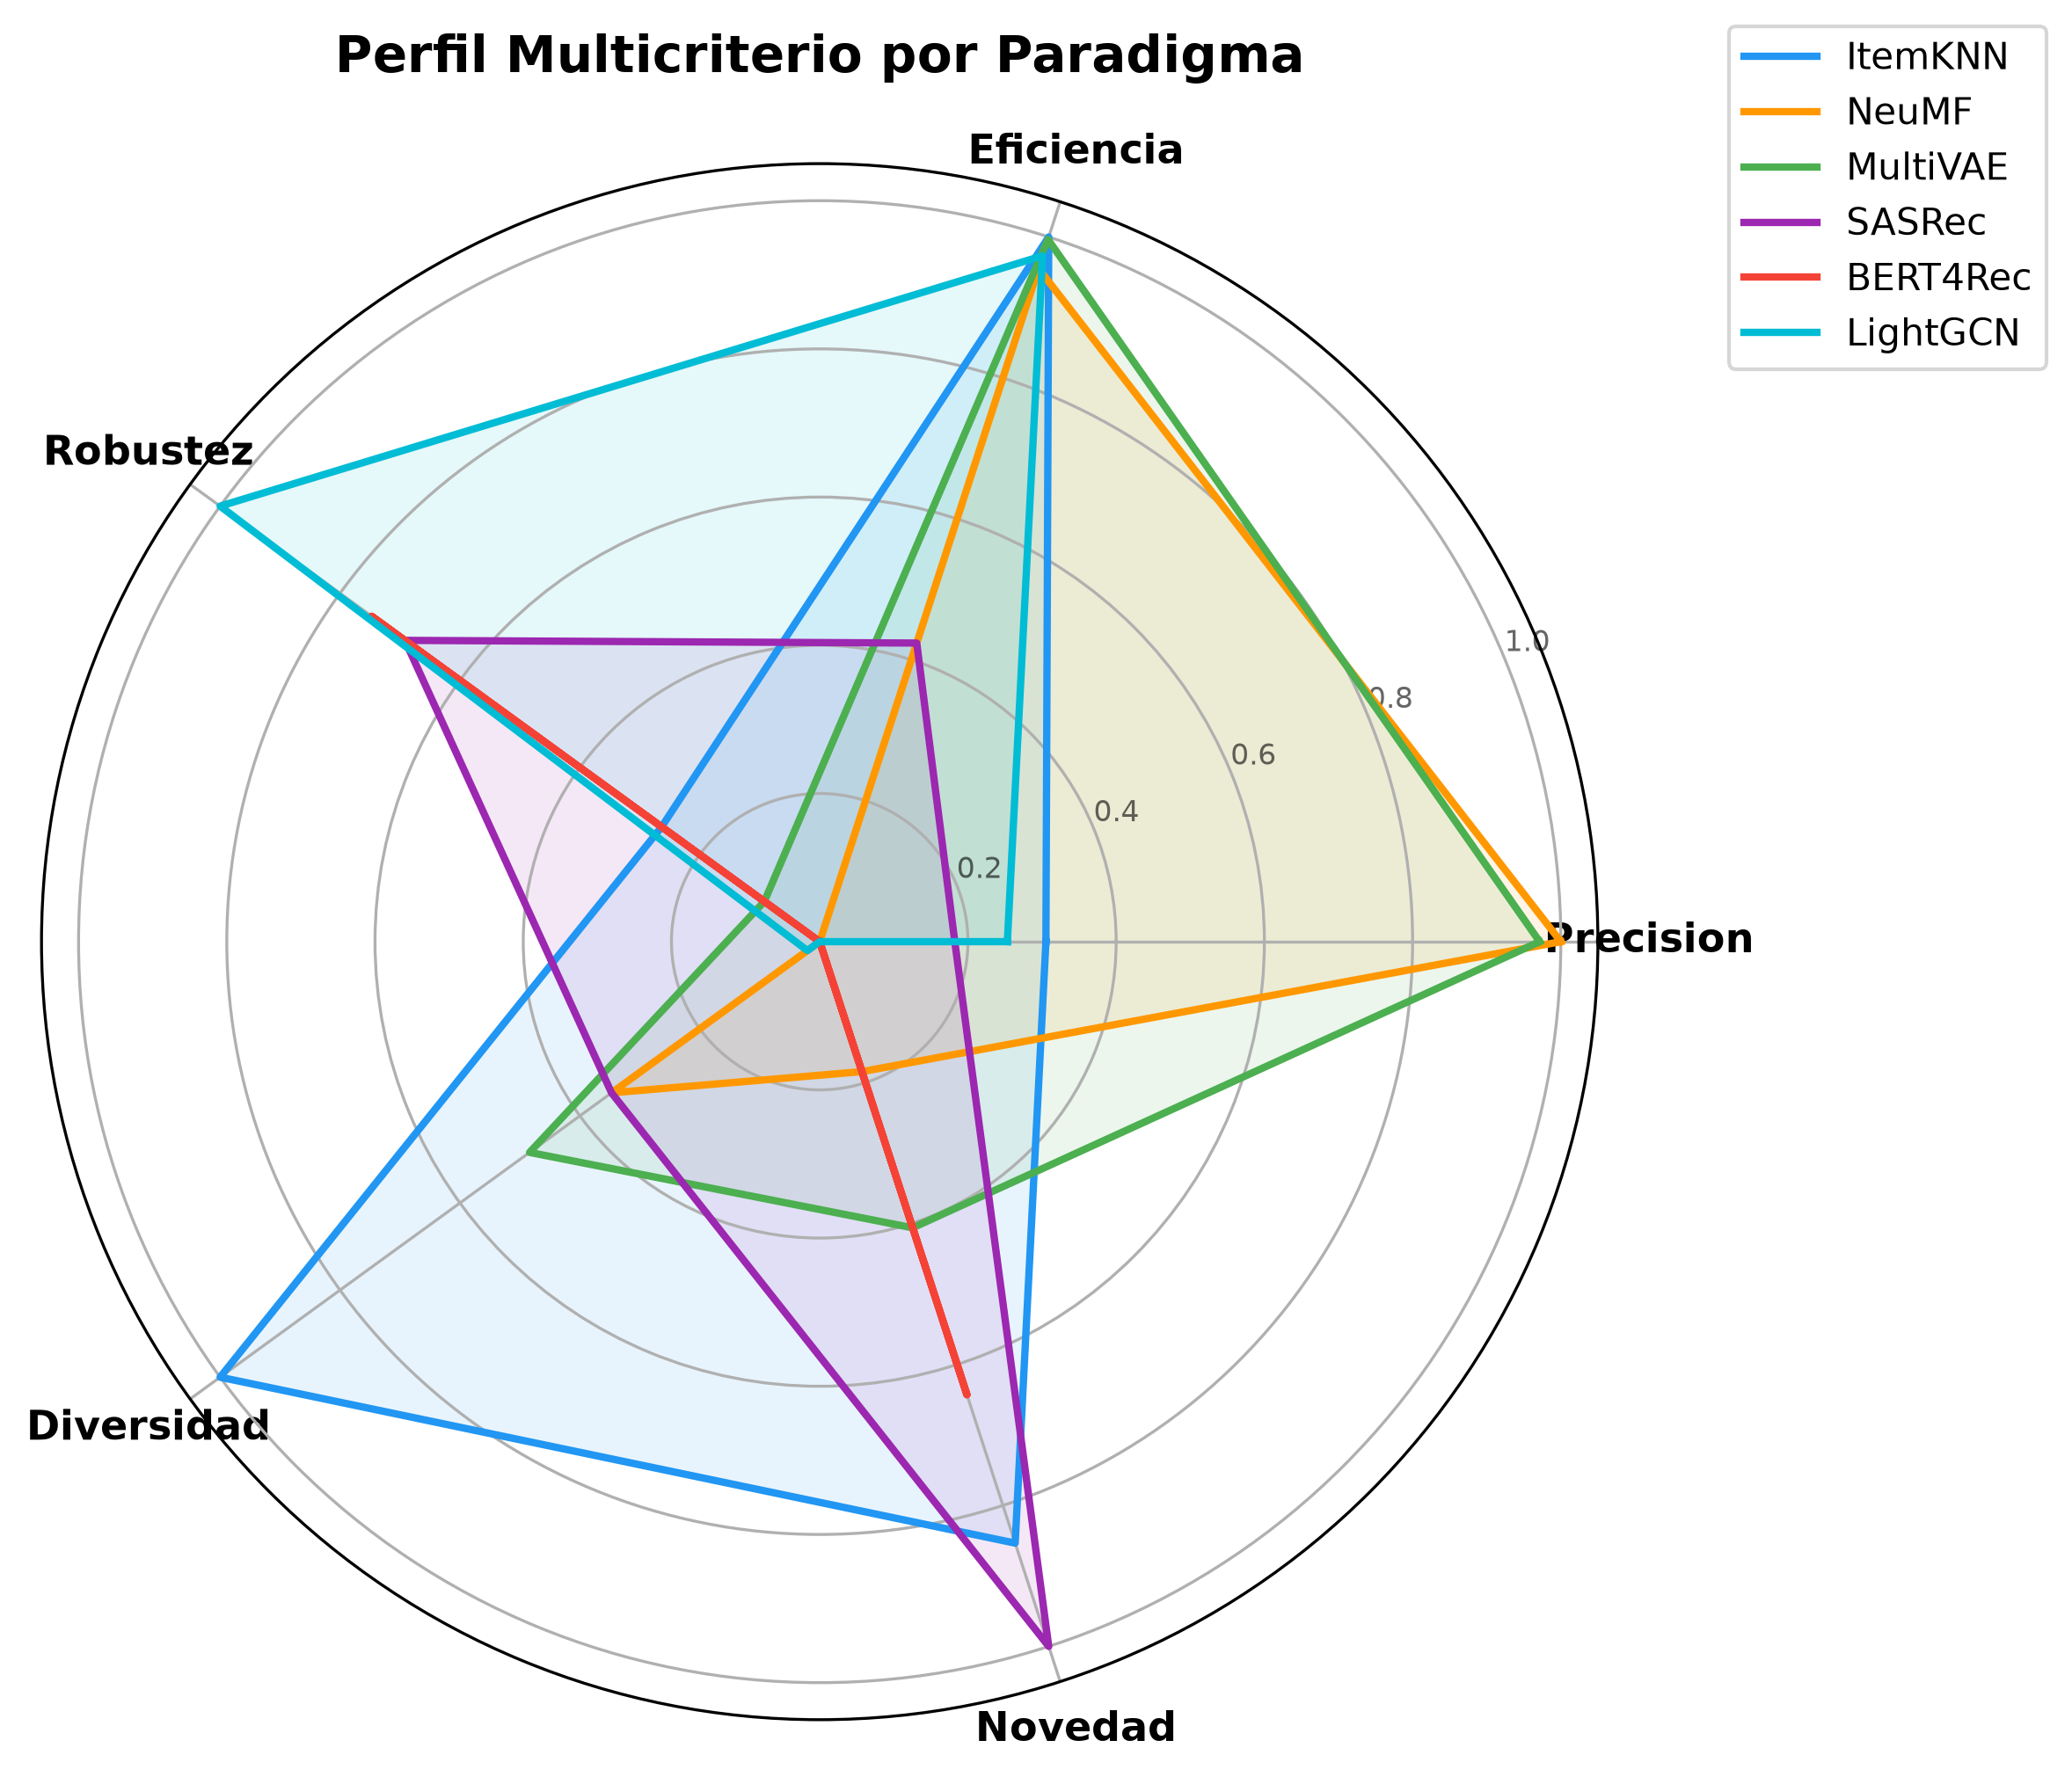
\includegraphics[width=0.45\textwidth]{figures/fig8_radar.png}
\caption{Perfil multi-criterio de los paradigmas en cinco dimensiones normalizadas.}
\label{fig:radar}
\end{figure}

\begin{figure}[h]
\centering
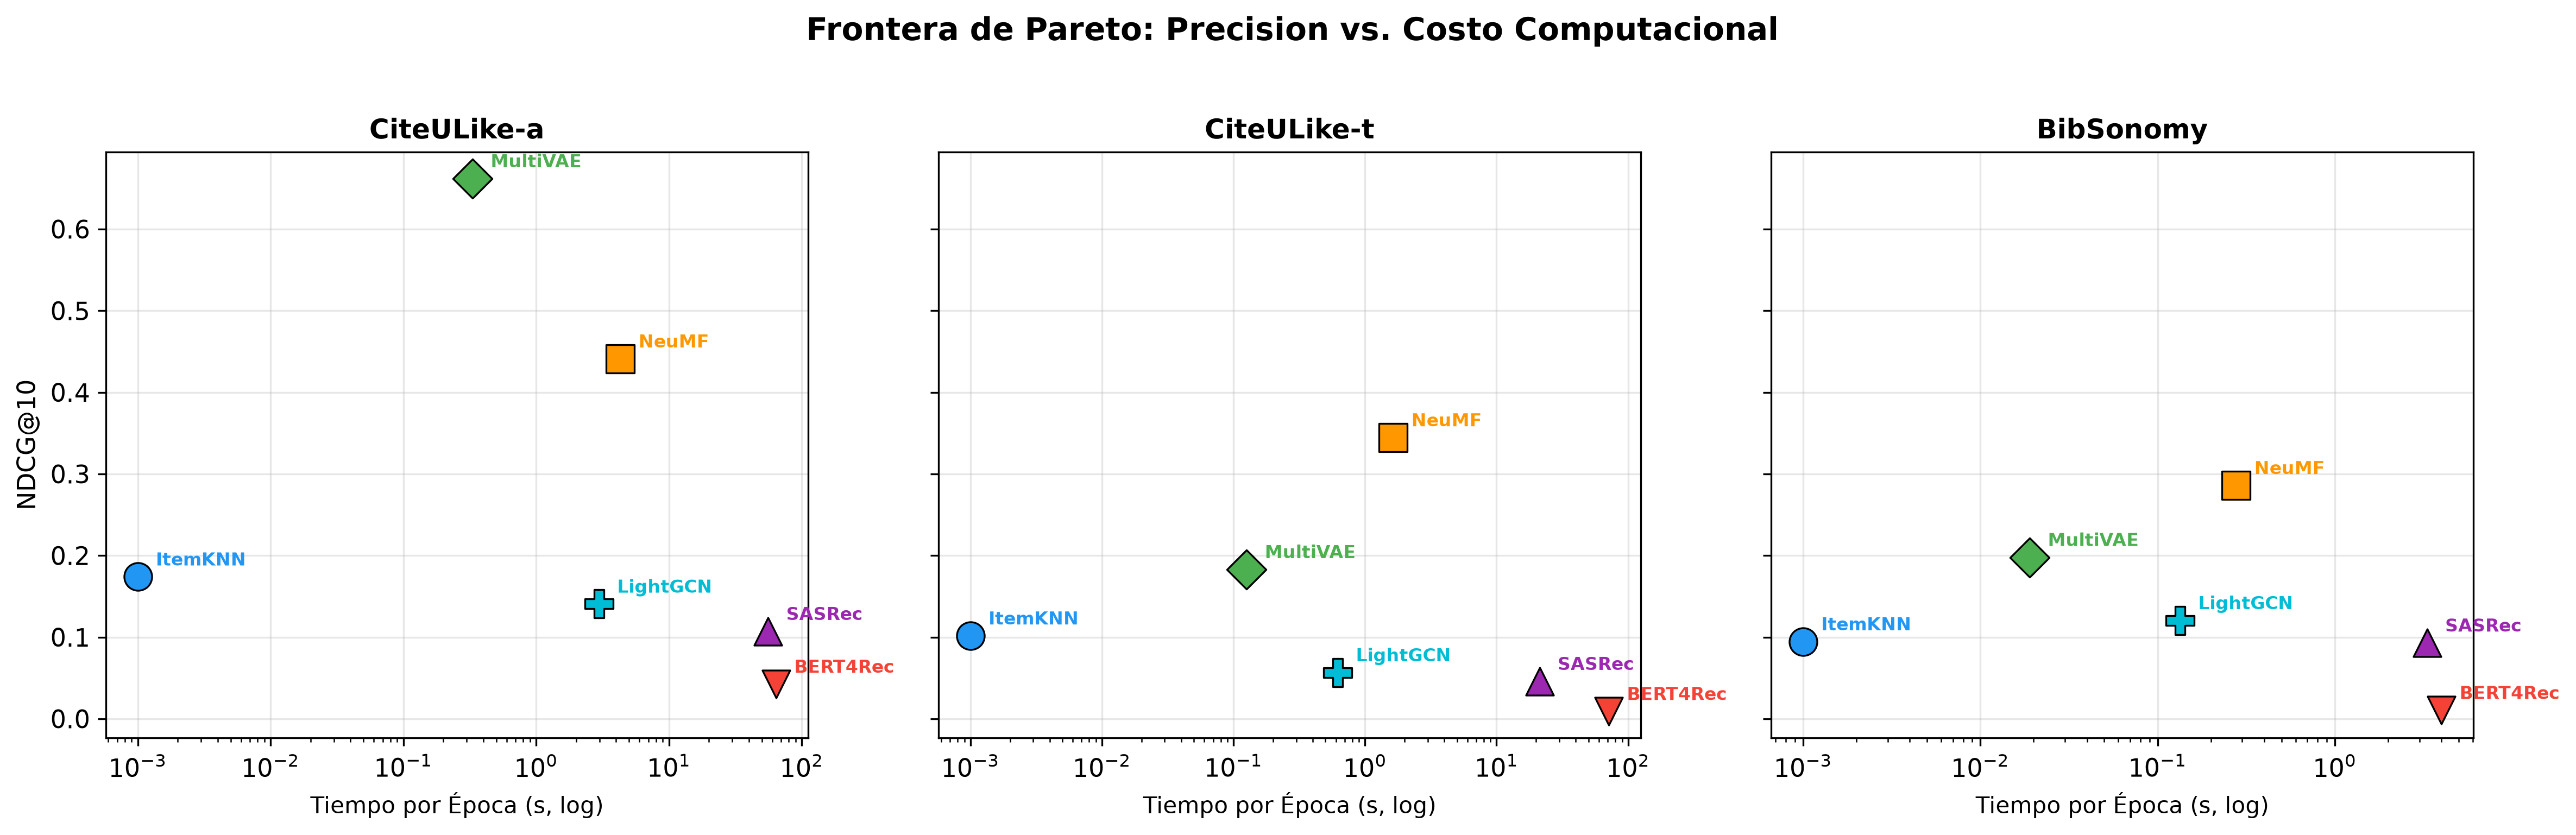
\includegraphics[width=0.45\textwidth]{figures/fig3_pareto.png}
\caption{Frontera de Pareto (NDCG\at{10} vs. Tiempo por Época) en los tres conjuntos de datos.}
\label{fig:pareto}
\end{figure}

El análisis de dominancia de Pareto sobre los datos del benchmark confirma que no existe un modelo óptimo universal:
\begin{enumerate}
    \item \textbf{MultiVAE:} Define el frente de Pareto no dominado en precisión offline en CiteULike-a (Recall\at{10} = 0.8143 en LOO y 0.7159 en RS).
    \item \textbf{ItemKNN:} Domina la frontera en cobertura de catálogo (ItemCoverage\at{10} = 0.8297) y eficiencia de entrenamiento nula (0.00 s/época).
    \item \textbf{LightGCN:} Domina la frontera en menor sensibilidad combinada ante la reducción drástica de datos al 20\%.
\end{enumerate}

% ==============================================================================
% 6. DISCUSIÓN Y AMENAZAS A LA VALIDEZ
% ==============================================================================
\section{Discusión y Amenazas a la Validez}
\label{sec:discusion}

\subsection{Criterios de Selección en Entornos Operativos}
La Tabla~\ref{tab:decision} resume recomendaciones prácticas de selección algorítmica orientadas a desarrolladores e ingenieros de plataformas académicas.

\begin{table}[H]
\centering
\caption{Guía de orientación para la selección de modelos en producción.}
\label{tab:decision}
\footnotesize
\setlength{\tabcolsep}{3pt}
\begin{tabular}{p{2.3cm}p{5.5cm}}
\toprule
\textbf{Restricción u Objetivo} & \textbf{Sugerencia Algorítmica y Justificación} \\
\midrule
Entornos limitados a CPU & \textbf{ItemKNN:} Operativo sin necesidad de GPU ni fase de entrenamiento. \\
Búsqueda de precisión offline & \textbf{MultiVAE / NeuMF:} Adecuados en colecciones con densidad suficiente de interacciones. \\
Diversidad y exploración & \textbf{ItemKNN / SASRec:} Generan recomendaciones con menor sesgo hacia artículos populares. \\
Sensibilidad a reducción de datos & \textbf{SASRec / LightGCN:} SASRec presenta la menor degradación ante reducciones moderadas (50\%), mientras que LightGCN exhibe la menor sensibilidad combinada ante reducción extrema (20\%). Nota: esta evaluación acopla escasez general y cold-start parcial (ver Sección~VI-B). \\
\bottomrule
\end{tabular}
\end{table}

\subsection{Amenazas a la Validez}

\subsubsection{Dependencia del Framework de Implementación}
Todos los experimentos se ejecutaron sobre RecBole~\cite{zhao2021recbole} bajo una semilla fija (2024). Las optimizaciones internas de tensores pueden variar en implementaciones independientes.

\subsubsection{Sensibilidad a la Partición Temporal en Modelos Secuenciales}
Los modelos secuenciales (SASRec y BERT4Rec) requieren por definición un esquema con ordenamiento temporal como Leave-One-Out (LOO) para alcanzar su máxima capacidad predictiva. Su evaluación bajo Random Split (RS) sirve como contraste para medir la pérdida de desempeño al destruir la secuencia de lectura.

\subsubsection{Sensibilidad a Hiperparámetros por Colección}
Se adoptaron configuraciones estándar basadas en las recomendaciones autorativas de los creadores de cada modelo. Una optimización de grilla bayesiana por dataset podría afinar marginalmente el rendimiento de ciertas redes profundas.

\subsubsection{Asimetría en la Calibración de ItemKNN}
\label{subsec:itemknn-tuning}
Los hiperparámetros de ItemKNN ($k=100$, $h=10$) se adoptaron de forma fija siguiendo las recomendaciones de la literatura~\cite{sarwar2001item}, sin búsqueda por dataset. En contraste, los modelos profundos disponen de early stopping adaptativo (paciencia de 10 épocas sobre 300 máximas), lo que les permite ajustar implícitamente la complejidad del modelo al volumen de cada colección. Esta asimetría de calibración podría sesgar la comparación en cualquier dirección: ItemKNN podría estar subóptimo (si valores distintos de $k$ o $h$ mejoraran su rendimiento en algún dataset) o favorecido (si los valores fijos coinciden favorablemente con la estructura de los datos evaluados). Aunque Dacrema et al.~\cite{dacrema2019really} recomiendan calibrar los baselines con el mismo rigor que los modelos profundos, el presente estudio priorizó la configuración canónica para asegurar la reproducibilidad directa con la literatura previa.

\subsubsection{Ausencia de Evaluación Online}
El estudio se acota a métricas offline. Aspectos de interacción real (como CTR o serendipia percibida) requieren pruebas A/B en producción.

\subsubsection{Limitación de Potencia Estadística en Bloques Independientes}
El tamaño del conjunto de bloques de observación independientes en la prueba de Friedman es de $N=6$ (3 conjuntos de datos $\times$ 2 protocolos). Aunque este número es adecuado para estructurar comparaciones robustas sin pseudo-replicación, impone límites sobre la potencia estadística de la prueba. En consecuencia, el valor de diferencia crítica de Nemenyi resulta relativamente conservador ($CD = 3.08$), permitiendo detectar significancia estadística formal únicamente ante diferencias extremas de rango (como MultiVAE/NeuMF contra BERT4Rec), e impidiendo que variaciones apreciables en las métricas de precisión offline alcancen significancia formal.

\subsubsection{Ausencia de Medición Dinámica de VRAM}
El consumo de memoria GPU (VRAM) para los recomendadores MultiVAE, NeuMF y LightGCN no fue instrumentado dinámicamente (marcados como ``n/m'' en la Tabla~\ref{tab:compute}), ya que los logs de RecBole no capturaron la memoria dinámica en tiempo de ejecución. Esto impide cuantificar el impacto diferencial del tamaño de los pesos y estados del optimizador (por ejemplo, los estados de Adam en MultiVAE con 18.6M parámetros frente a LightGCN con 1.3M), representando una amenaza a la validez interna del análisis de costo computacional.

\subsubsection{Varianza Estocástica y Ausencia de Múltiples Semillas}
Para asegurar la reproducibilidad determinista y acotar el costo computacional de evaluar 36 condiciones con modelos pesados, todos los experimentos se ejecutaron bajo una semilla fija única (2024). Esto constituye una amenaza a la validez interna, ya que el rendimiento relativo de los recomendadores estocásticos (como MultiVAE con muestreo variacional, y NeuMF o SASRec con inicialización aleatoria de pesos y dropout) podría verse afectado por la varianza de entrenamiento de la semilla seleccionada, imposibilitando separar la variabilidad de inicialización de la superioridad algorítmica intrínseca.

\subsubsection{Ruptura de la Invariante 5-Core en el Submuestreo de Entrenamiento}
\label{subsec:ruptura-5core}
Al evaluar la robustez (RQ3) reduciendo los datos de entrenamiento al 50\% y 20\%, no se re-aplicó el filtrado iterativo 5-core sobre el subset resultante. Esto representa una amenaza a la validez interna, ya que rompe la restricción 5-core de forma local e induce cold-start parcial (usuarios o ítems con soporte extremadamente bajo en entrenamiento), mientras el conjunto de prueba permanece fijo. Por lo tanto, la robustez reportada podría estar midiendo de forma combinada la tolerancia a la escasez general y la resiliencia al cold-start parcial inducido.

\subsubsection{Variabilidad por Throttling Térmico en Hardware de Consumo}
Las mediciones de costo computacional (tiempo por época y throughput) se realizaron en una estación de trabajo equipada con una GPU de laptop (RTX 3050 Laptop). A pesar de mantener condiciones ambientales estables, el hardware móvil es susceptible a fenómenos de estrangulamiento térmico (thermal throttling) bajo cargas prolongadas de trabajo. Esto representa una amenaza a la precisión temporal reportada, pudiendo introducir fluctuaciones menores en los tiempos por época.

\subsubsection{Limitaciones de Validez Externa}
Los resultados aplican al dominio de marcadores académicos (CiteULike, BibSonomy) y no deben ser extrapolados directamente a comercio electrónico o streaming.

% ==============================================================================
% 7. CONCLUSIÓN Y TRABAJO FUTURO
% ==============================================================================
\section{Conclusión y Trabajo Futuro}
\label{sec:conclusion}

Este estudio presentó un benchmark multi-criterio de seis paradigmas de recomendación sobre tres conjuntos de datos académicos. Los resultados confirman que la precisión offline (NDCG, Recall) debe ser ponderada junto a la eficiencia computacional, la diversidad y la robustez ante la escasez de datos. Como trabajo futuro, se plantea la integración de Modelos de Lenguaje de Gran Escala (LLMs) para mitigar el arranque en frío mediante representaciones semánticas de resúmenes científicos.

\section*{Disponibilidad de Datos y Código}
Para asegurar la reproducibilidad completa de este benchmark, todos los archivos de configuración, scripts de preprocesamiento, de entrenamiento, pesos de modelos entrenados y los reportes de resultados crudos se encuentran disponibles de manera pública en el repositorio de GitHub de la investigación en \url{https://github.com/XavierPenaA/scientific-paper-recommendation-benchmark}. El estado exacto del código correspondiente a los resultados reportados se identifica mediante el tag \texttt{v1.0-benchmark} del repositorio.

% ==============================================================================
% REFERENCIAS
% ==============================================================================
\section*{Agradecimientos}
Los autores agradecen el uso de sistemas de inteligencia artificial, específicamente Gemini 3.5 Flash de Google DeepMind~\cite{gemini2026} y Claude Opus 4.6 de Anthropic~\cite{claude2026}, para asistir en la traducción, revisión gramatical y pulido estilístico de este manuscrito.

\bibliographystyle{IEEEtran}
\bibliography{references}

\begin{IEEEbiographynophoto}{Xavier Peña}
recibió el título de Ingeniero en Computación de la Universidad de Cuenca, Cuenca, Ecuador. Sus áreas de interés en investigación incluyen el filtrado colaborativo, los sistemas de recomendación, el aprendizaje de máquina y la reproducibilidad de arquitecturas de redes neuronales aplicadas a la recomendación de literatura académica.
\end{IEEEbiographynophoto}

\begin{IEEEbiographynophoto}{Diego Rivera}
es investigador y docente en la Universidad Politécnica Salesiana, Cuenca, Ecuador. Se desempeña como Vicepresidente de la Sociedad de Tecnología Vehicular (VTS) de IEEE Sección Ecuador. Sus áreas de interés en investigación abarcan las redes vehiculares, ciudades inteligentes, sistemas de recomendación y aprendizaje de máquina aplicado.
\end{IEEEbiographynophoto}


\EOD

\end{document}
